% Created by tikzDevice version 0.7.0 on 2014-07-01 19:29:08
% !TEX encoding = UTF-8 Unicode
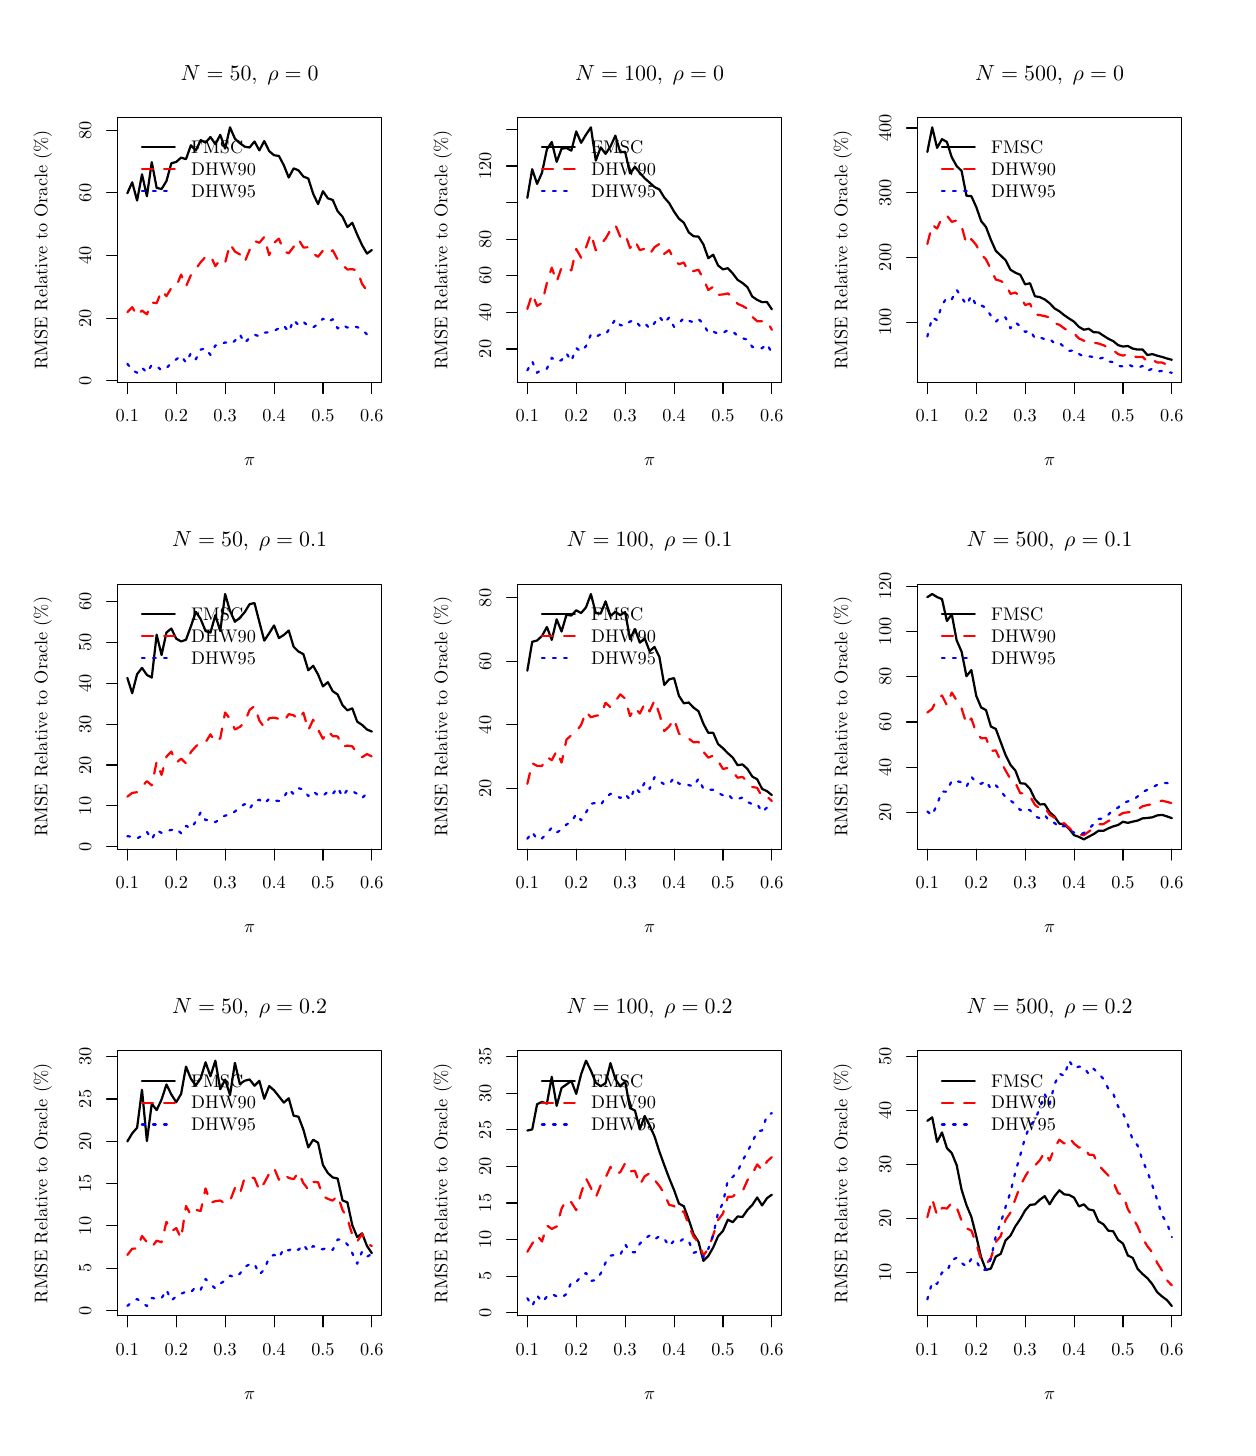
\begin{tikzpicture}[x=1pt,y=1pt]
\definecolor[named]{fillColor}{rgb}{1.00,1.00,1.00}
\path[use as bounding box,fill=fillColor,fill opacity=0.00] (0,0) rectangle (433.62,505.89);
\begin{scope}
\path[clip] ( 32.47,377.65) rectangle (127.91,473.42);
\definecolor[named]{drawColor}{rgb}{0.00,0.00,0.00}

\path[draw=drawColor,line width= 0.8pt,line join=round,line cap=round] ( 36.01,446.04) --
	( 37.77,450.01) --
	( 39.54,443.42) --
	( 41.31,452.91) --
	( 43.08,444.98) --
	( 44.84,457.29) --
	( 46.61,447.99) --
	( 48.38,447.58) --
	( 50.15,450.47) --
	( 51.91,456.88) --
	( 53.68,457.37) --
	( 55.45,458.94) --
	( 57.21,458.37) --
	( 58.98,463.40) --
	( 60.75,461.47) --
	( 62.52,465.25) --
	( 64.28,464.34) --
	( 66.05,466.38) --
	( 67.82,463.79) --
	( 69.59,467.15) --
	( 71.35,462.19) --
	( 73.12,469.87) --
	( 74.89,465.76) --
	( 76.66,464.17) --
	( 78.42,462.89) --
	( 80.19,462.59) --
	( 81.96,464.75) --
	( 83.72,461.54) --
	( 85.49,464.90) --
	( 87.26,461.28) --
	( 89.03,459.79) --
	( 90.79,459.53) --
	( 92.56,456.17) --
	( 94.33,451.73) --
	( 96.10,455.04) --
	( 97.86,454.33) --
	( 99.63,452.09) --
	(101.40,451.38) --
	(103.17,445.85) --
	(104.93,442.12) --
	(106.70,446.78) --
	(108.47,444.23) --
	(110.23,443.64) --
	(112.00,439.56) --
	(113.77,437.56) --
	(115.54,433.81) --
	(117.30,435.37) --
	(119.07,431.13) --
	(120.84,427.30) --
	(122.61,424.25) --
	(124.37,425.53);
\end{scope}
\begin{scope}
\path[clip] (  0.00,  0.00) rectangle (433.62,505.89);
\definecolor[named]{drawColor}{rgb}{0.00,0.00,0.00}

\path[draw=drawColor,line width= 0.4pt,line join=round,line cap=round] ( 36.01,377.65) -- (124.37,377.65);

\path[draw=drawColor,line width= 0.4pt,line join=round,line cap=round] ( 36.01,377.65) -- ( 36.01,373.69);

\path[draw=drawColor,line width= 0.4pt,line join=round,line cap=round] ( 53.68,377.65) -- ( 53.68,373.69);

\path[draw=drawColor,line width= 0.4pt,line join=round,line cap=round] ( 71.35,377.65) -- ( 71.35,373.69);

\path[draw=drawColor,line width= 0.4pt,line join=round,line cap=round] ( 89.03,377.65) -- ( 89.03,373.69);

\path[draw=drawColor,line width= 0.4pt,line join=round,line cap=round] (106.70,377.65) -- (106.70,373.69);

\path[draw=drawColor,line width= 0.4pt,line join=round,line cap=round] (124.37,377.65) -- (124.37,373.69);

\node[text=drawColor,anchor=base,inner sep=0pt, outer sep=0pt, scale=  0.66] at ( 36.01,363.40) {0.1};

\node[text=drawColor,anchor=base,inner sep=0pt, outer sep=0pt, scale=  0.66] at ( 53.68,363.40) {0.2};

\node[text=drawColor,anchor=base,inner sep=0pt, outer sep=0pt, scale=  0.66] at ( 71.35,363.40) {0.3};

\node[text=drawColor,anchor=base,inner sep=0pt, outer sep=0pt, scale=  0.66] at ( 89.03,363.40) {0.4};

\node[text=drawColor,anchor=base,inner sep=0pt, outer sep=0pt, scale=  0.66] at (106.70,363.40) {0.5};

\node[text=drawColor,anchor=base,inner sep=0pt, outer sep=0pt, scale=  0.66] at (124.37,363.40) {0.6};

\path[draw=drawColor,line width= 0.4pt,line join=round,line cap=round] ( 32.47,378.33) -- ( 32.47,468.79);

\path[draw=drawColor,line width= 0.4pt,line join=round,line cap=round] ( 32.47,378.33) -- ( 28.51,378.33);

\path[draw=drawColor,line width= 0.4pt,line join=round,line cap=round] ( 32.47,400.95) -- ( 28.51,400.95);

\path[draw=drawColor,line width= 0.4pt,line join=round,line cap=round] ( 32.47,423.56) -- ( 28.51,423.56);

\path[draw=drawColor,line width= 0.4pt,line join=round,line cap=round] ( 32.47,446.18) -- ( 28.51,446.18);

\path[draw=drawColor,line width= 0.4pt,line join=round,line cap=round] ( 32.47,468.79) -- ( 28.51,468.79);

\node[text=drawColor,rotate= 90.00,anchor=base,inner sep=0pt, outer sep=0pt, scale=  0.66] at ( 22.97,378.33) {0};

\node[text=drawColor,rotate= 90.00,anchor=base,inner sep=0pt, outer sep=0pt, scale=  0.66] at ( 22.97,400.95) {20};

\node[text=drawColor,rotate= 90.00,anchor=base,inner sep=0pt, outer sep=0pt, scale=  0.66] at ( 22.97,423.56) {40};

\node[text=drawColor,rotate= 90.00,anchor=base,inner sep=0pt, outer sep=0pt, scale=  0.66] at ( 22.97,446.18) {60};

\node[text=drawColor,rotate= 90.00,anchor=base,inner sep=0pt, outer sep=0pt, scale=  0.66] at ( 22.97,468.79) {80};

\path[draw=drawColor,line width= 0.4pt,line join=round,line cap=round] ( 32.47,377.65) --
	(127.91,377.65) --
	(127.91,473.42) --
	( 32.47,473.42) --
	( 32.47,377.65);
\end{scope}
\begin{scope}
\path[clip] (  0.00,337.26) rectangle (144.54,505.89);
\definecolor[named]{drawColor}{rgb}{0.00,0.00,0.00}

\node[text=drawColor,anchor=base,inner sep=0pt, outer sep=0pt, scale=  0.79] at ( 80.19,486.92) {\bfseries $N=50, \;\rho=0$};

\node[text=drawColor,anchor=base,inner sep=0pt, outer sep=0pt, scale=  0.66] at ( 80.19,347.56) {$\pi$};

\node[text=drawColor,rotate= 90.00,anchor=base,inner sep=0pt, outer sep=0pt, scale=  0.66] at (  7.13,425.53) {RMSE Relative to Oracle (\%)};
\end{scope}
\begin{scope}
\path[clip] ( 32.47,377.65) rectangle (127.91,473.42);
\definecolor[named]{drawColor}{rgb}{1.00,0.00,0.00}

\path[draw=drawColor,line width= 0.8pt,dash pattern=on 4pt off 4pt ,line join=round,line cap=round] ( 36.01,403.05) --
	( 37.77,404.89) --
	( 39.54,401.81) --
	( 41.31,403.68) --
	( 43.08,402.29) --
	( 44.84,406.58) --
	( 46.61,406.33) --
	( 48.38,410.90) --
	( 50.15,408.87) --
	( 51.91,411.83) --
	( 53.68,412.36) --
	( 55.45,416.66) --
	( 57.21,412.36) --
	( 58.98,416.49) --
	( 60.75,418.67) --
	( 62.52,421.15) --
	( 64.28,423.06) --
	( 66.05,423.59) --
	( 67.82,419.71) --
	( 69.59,422.09) --
	( 71.35,420.98) --
	( 73.12,427.73) --
	( 74.89,424.99) --
	( 76.66,423.95) --
	( 78.42,421.24) --
	( 80.19,425.55) --
	( 81.96,428.80) --
	( 83.72,428.16) --
	( 85.49,430.27) --
	( 87.26,423.68) --
	( 89.03,428.10) --
	( 90.79,429.65) --
	( 92.56,425.08) --
	( 94.33,424.37) --
	( 96.10,426.69) --
	( 97.86,429.43) --
	( 99.63,426.47) --
	(101.40,426.51) --
	(103.17,424.22) --
	(104.93,423.09) --
	(106.70,425.38) --
	(108.47,424.17) --
	(110.23,425.44) --
	(112.00,422.13) --
	(113.77,420.11) --
	(115.54,418.51) --
	(117.30,418.61) --
	(119.07,418.17) --
	(120.84,413.28) --
	(122.61,410.85) --
	(124.37,412.71);
\definecolor[named]{drawColor}{rgb}{0.00,0.00,1.00}

\path[draw=drawColor,line width= 0.8pt,dash pattern=on 1pt off 3pt ,line join=round,line cap=round] ( 36.01,384.45) --
	( 37.77,382.14) --
	( 39.54,381.20) --
	( 41.31,383.07) --
	( 43.08,381.22) --
	( 44.84,384.04) --
	( 46.61,383.60) --
	( 48.38,382.04) --
	( 50.15,382.81) --
	( 51.91,384.80) --
	( 53.68,386.03) --
	( 55.45,387.33) --
	( 57.21,384.88) --
	( 58.98,388.28) --
	( 60.75,386.07) --
	( 62.52,389.54) --
	( 64.28,390.04) --
	( 66.05,387.63) --
	( 67.82,391.05) --
	( 69.59,391.11) --
	( 71.35,392.19) --
	( 73.12,391.54) --
	( 74.89,392.74) --
	( 76.66,395.05) --
	( 78.42,391.94) --
	( 80.19,393.85) --
	( 81.96,394.93) --
	( 83.72,394.38) --
	( 85.49,395.66) --
	( 87.26,395.85) --
	( 89.03,396.36) --
	( 90.79,397.25) --
	( 92.56,398.22) --
	( 94.33,395.98) --
	( 96.10,400.30) --
	( 97.86,398.39) --
	( 99.63,399.59) --
	(101.40,398.01) --
	(103.17,397.59) --
	(104.93,398.82) --
	(106.70,400.75) --
	(108.47,399.50) --
	(110.23,400.53) --
	(112.00,397.20) --
	(113.77,398.51) --
	(115.54,397.51) --
	(117.30,398.11) --
	(119.07,397.68) --
	(120.84,396.96) --
	(122.61,395.01) --
	(124.37,394.61);
\definecolor[named]{drawColor}{rgb}{0.00,0.00,0.00}

\path[draw=drawColor,line width= 0.8pt,line join=round,line cap=round] ( 41.28,462.63) -- ( 53.16,462.63);
\definecolor[named]{drawColor}{rgb}{1.00,0.00,0.00}

\path[draw=drawColor,line width= 0.8pt,dash pattern=on 4pt off 4pt ,line join=round,line cap=round] ( 41.28,454.71) -- ( 53.16,454.71);
\definecolor[named]{drawColor}{rgb}{0.00,0.00,1.00}

\path[draw=drawColor,line width= 0.8pt,dash pattern=on 1pt off 3pt ,line join=round,line cap=round] ( 41.28,446.79) -- ( 53.16,446.79);
\definecolor[named]{drawColor}{rgb}{0.00,0.00,0.00}

\node[text=drawColor,anchor=base west,inner sep=0pt, outer sep=0pt, scale=  0.66] at ( 59.10,460.35) {FMSC};

\node[text=drawColor,anchor=base west,inner sep=0pt, outer sep=0pt, scale=  0.66] at ( 59.10,452.43) {DHW90};

\node[text=drawColor,anchor=base west,inner sep=0pt, outer sep=0pt, scale=  0.66] at ( 59.10,444.51) {DHW95};
\end{scope}
\begin{scope}
\path[clip] (177.01,377.65) rectangle (272.45,473.42);
\definecolor[named]{drawColor}{rgb}{0.00,0.00,0.00}

\path[draw=drawColor,line width= 0.8pt,line join=round,line cap=round] (180.55,444.38) --
	(182.31,454.74) --
	(184.08,449.44) --
	(185.85,453.47) --
	(187.62,461.92) --
	(189.38,464.57) --
	(191.15,457.39) --
	(192.92,462.14) --
	(194.69,462.42) --
	(196.45,461.43) --
	(198.22,468.41) --
	(199.99,464.26) --
	(201.75,467.24) --
	(203.52,469.87) --
	(205.29,457.86) --
	(207.06,462.64) --
	(208.82,460.29) --
	(210.59,462.93) --
	(212.36,466.86) --
	(214.13,460.87) --
	(215.89,461.03) --
	(217.66,453.24) --
	(219.43,455.60) --
	(221.20,453.43) --
	(222.96,451.45) --
	(224.73,449.91) --
	(226.50,448.31) --
	(228.26,447.41) --
	(230.03,444.51) --
	(231.80,442.49) --
	(233.57,439.42) --
	(235.33,436.88) --
	(237.10,435.41) --
	(238.87,431.91) --
	(240.64,430.51) --
	(242.40,430.38) --
	(244.17,427.56) --
	(245.94,422.58) --
	(247.71,423.84) --
	(249.47,419.97) --
	(251.24,418.53) --
	(253.01,418.97) --
	(254.77,417.08) --
	(256.54,414.75) --
	(258.31,413.62) --
	(260.08,412.11) --
	(261.84,408.71) --
	(263.61,407.52) --
	(265.38,406.70) --
	(267.15,406.74) --
	(268.91,404.09);
\end{scope}
\begin{scope}
\path[clip] (  0.00,  0.00) rectangle (433.62,505.89);
\definecolor[named]{drawColor}{rgb}{0.00,0.00,0.00}

\path[draw=drawColor,line width= 0.4pt,line join=round,line cap=round] (180.55,377.65) -- (268.91,377.65);

\path[draw=drawColor,line width= 0.4pt,line join=round,line cap=round] (180.55,377.65) -- (180.55,373.69);

\path[draw=drawColor,line width= 0.4pt,line join=round,line cap=round] (198.22,377.65) -- (198.22,373.69);

\path[draw=drawColor,line width= 0.4pt,line join=round,line cap=round] (215.89,377.65) -- (215.89,373.69);

\path[draw=drawColor,line width= 0.4pt,line join=round,line cap=round] (233.57,377.65) -- (233.57,373.69);

\path[draw=drawColor,line width= 0.4pt,line join=round,line cap=round] (251.24,377.65) -- (251.24,373.69);

\path[draw=drawColor,line width= 0.4pt,line join=round,line cap=round] (268.91,377.65) -- (268.91,373.69);

\node[text=drawColor,anchor=base,inner sep=0pt, outer sep=0pt, scale=  0.66] at (180.55,363.40) {0.1};

\node[text=drawColor,anchor=base,inner sep=0pt, outer sep=0pt, scale=  0.66] at (198.22,363.40) {0.2};

\node[text=drawColor,anchor=base,inner sep=0pt, outer sep=0pt, scale=  0.66] at (215.89,363.40) {0.3};

\node[text=drawColor,anchor=base,inner sep=0pt, outer sep=0pt, scale=  0.66] at (233.57,363.40) {0.4};

\node[text=drawColor,anchor=base,inner sep=0pt, outer sep=0pt, scale=  0.66] at (251.24,363.40) {0.5};

\node[text=drawColor,anchor=base,inner sep=0pt, outer sep=0pt, scale=  0.66] at (268.91,363.40) {0.6};

\path[draw=drawColor,line width= 0.4pt,line join=round,line cap=round] (177.01,389.78) -- (177.01,469.12);

\path[draw=drawColor,line width= 0.4pt,line join=round,line cap=round] (177.01,389.78) -- (173.05,389.78);

\path[draw=drawColor,line width= 0.4pt,line join=round,line cap=round] (177.01,403.00) -- (173.05,403.00);

\path[draw=drawColor,line width= 0.4pt,line join=round,line cap=round] (177.01,416.23) -- (173.05,416.23);

\path[draw=drawColor,line width= 0.4pt,line join=round,line cap=round] (177.01,429.45) -- (173.05,429.45);

\path[draw=drawColor,line width= 0.4pt,line join=round,line cap=round] (177.01,442.67) -- (173.05,442.67);

\path[draw=drawColor,line width= 0.4pt,line join=round,line cap=round] (177.01,455.90) -- (173.05,455.90);

\path[draw=drawColor,line width= 0.4pt,line join=round,line cap=round] (177.01,469.12) -- (173.05,469.12);

\node[text=drawColor,rotate= 90.00,anchor=base,inner sep=0pt, outer sep=0pt, scale=  0.66] at (167.51,389.78) {20};

\node[text=drawColor,rotate= 90.00,anchor=base,inner sep=0pt, outer sep=0pt, scale=  0.66] at (167.51,403.00) {40};

\node[text=drawColor,rotate= 90.00,anchor=base,inner sep=0pt, outer sep=0pt, scale=  0.66] at (167.51,416.23) {60};

\node[text=drawColor,rotate= 90.00,anchor=base,inner sep=0pt, outer sep=0pt, scale=  0.66] at (167.51,429.45) {80};

\node[text=drawColor,rotate= 90.00,anchor=base,inner sep=0pt, outer sep=0pt, scale=  0.66] at (167.51,455.90) {120};

\path[draw=drawColor,line width= 0.4pt,line join=round,line cap=round] (177.01,377.65) --
	(272.45,377.65) --
	(272.45,473.42) --
	(177.01,473.42) --
	(177.01,377.65);
\end{scope}
\begin{scope}
\path[clip] (144.54,337.26) rectangle (289.08,505.89);
\definecolor[named]{drawColor}{rgb}{0.00,0.00,0.00}

\node[text=drawColor,anchor=base,inner sep=0pt, outer sep=0pt, scale=  0.79] at (224.73,486.92) {\bfseries $N=100, \;\rho=0$};

\node[text=drawColor,anchor=base,inner sep=0pt, outer sep=0pt, scale=  0.66] at (224.73,347.56) {$\pi$};

\node[text=drawColor,rotate= 90.00,anchor=base,inner sep=0pt, outer sep=0pt, scale=  0.66] at (151.67,425.53) {RMSE Relative to Oracle (\%)};
\end{scope}
\begin{scope}
\path[clip] (177.01,377.65) rectangle (272.45,473.42);
\definecolor[named]{drawColor}{rgb}{1.00,0.00,0.00}

\path[draw=drawColor,line width= 0.8pt,dash pattern=on 4pt off 4pt ,line join=round,line cap=round] (180.55,404.24) --
	(182.31,409.69) --
	(184.08,405.35) --
	(185.85,406.40) --
	(187.62,413.60) --
	(189.38,419.16) --
	(191.15,414.07) --
	(192.92,419.19) --
	(194.69,419.28) --
	(196.45,418.16) --
	(198.22,425.92) --
	(199.99,422.77) --
	(201.75,426.47) --
	(203.52,431.47) --
	(205.29,425.42) --
	(207.06,427.59) --
	(208.82,429.66) --
	(210.59,432.74) --
	(212.36,434.67) --
	(214.13,430.34) --
	(215.89,431.35) --
	(217.66,426.27) --
	(219.43,428.85) --
	(221.20,425.49) --
	(222.96,426.02) --
	(224.73,423.99) --
	(226.50,426.54) --
	(228.26,427.74) --
	(230.03,424.16) --
	(231.80,425.50) --
	(233.57,422.18) --
	(235.33,420.40) --
	(237.10,421.02) --
	(238.87,417.51) --
	(240.64,417.95) --
	(242.40,418.40) --
	(244.17,415.07) --
	(245.94,411.10) --
	(247.71,412.26) --
	(249.47,409.34) --
	(251.24,409.48) --
	(253.01,409.85) --
	(254.77,408.49) --
	(256.54,406.08) --
	(258.31,405.34) --
	(260.08,404.31) --
	(261.84,401.40) --
	(263.61,399.80) --
	(265.38,399.80) --
	(267.15,399.88) --
	(268.91,396.70);
\definecolor[named]{drawColor}{rgb}{0.00,0.00,1.00}

\path[draw=drawColor,line width= 0.8pt,dash pattern=on 1pt off 3pt ,line join=round,line cap=round] (180.55,382.06) --
	(182.31,385.33) --
	(184.08,381.20) --
	(185.85,382.38) --
	(187.62,382.66) --
	(189.38,386.59) --
	(191.15,385.22) --
	(192.92,385.74) --
	(194.69,388.21) --
	(196.45,385.40) --
	(198.22,390.11) --
	(199.99,388.84) --
	(201.75,390.80) --
	(203.52,395.02) --
	(205.29,394.14) --
	(207.06,395.12) --
	(208.82,395.01) --
	(210.59,397.61) --
	(212.36,400.53) --
	(214.13,398.37) --
	(215.89,398.20) --
	(217.66,399.70) --
	(219.43,400.19) --
	(221.20,398.10) --
	(222.96,399.20) --
	(224.73,397.18) --
	(226.50,399.15) --
	(228.26,401.50) --
	(230.03,399.14) --
	(231.80,401.18) --
	(233.57,397.78) --
	(235.33,399.06) --
	(237.10,400.98) --
	(238.87,399.98) --
	(240.64,399.44) --
	(242.40,400.63) --
	(244.17,398.84) --
	(245.94,395.62) --
	(247.71,396.07) --
	(249.47,395.28) --
	(251.24,395.64) --
	(253.01,396.57) --
	(254.77,396.15) --
	(256.54,394.45) --
	(258.31,393.65) --
	(260.08,393.16) --
	(261.84,390.53) --
	(263.61,390.06) --
	(265.38,390.06) --
	(267.15,391.59) --
	(268.91,388.27);
\definecolor[named]{drawColor}{rgb}{0.00,0.00,0.00}

\path[draw=drawColor,line width= 0.8pt,line join=round,line cap=round] (185.82,462.63) -- (197.70,462.63);
\definecolor[named]{drawColor}{rgb}{1.00,0.00,0.00}

\path[draw=drawColor,line width= 0.8pt,dash pattern=on 4pt off 4pt ,line join=round,line cap=round] (185.82,454.71) -- (197.70,454.71);
\definecolor[named]{drawColor}{rgb}{0.00,0.00,1.00}

\path[draw=drawColor,line width= 0.8pt,dash pattern=on 1pt off 3pt ,line join=round,line cap=round] (185.82,446.79) -- (197.70,446.79);
\definecolor[named]{drawColor}{rgb}{0.00,0.00,0.00}

\node[text=drawColor,anchor=base west,inner sep=0pt, outer sep=0pt, scale=  0.66] at (203.64,460.35) {FMSC};

\node[text=drawColor,anchor=base west,inner sep=0pt, outer sep=0pt, scale=  0.66] at (203.64,452.43) {DHW90};

\node[text=drawColor,anchor=base west,inner sep=0pt, outer sep=0pt, scale=  0.66] at (203.64,444.51) {DHW95};
\end{scope}
\begin{scope}
\path[clip] (321.55,377.65) rectangle (416.99,473.42);
\definecolor[named]{drawColor}{rgb}{0.00,0.00,0.00}

\path[draw=drawColor,line width= 0.8pt,line join=round,line cap=round] (325.09,460.96) --
	(326.85,469.87) --
	(328.62,462.44) --
	(330.39,465.62) --
	(332.16,464.57) --
	(333.92,459.04) --
	(335.69,455.85) --
	(337.46,454.15) --
	(339.23,445.15) --
	(340.99,445.01) --
	(342.76,441.11) --
	(344.53,436.00) --
	(346.29,433.84) --
	(348.06,429.21) --
	(349.83,425.24) --
	(351.60,423.56) --
	(353.36,421.87) --
	(355.13,418.42) --
	(356.90,417.34) --
	(358.67,416.58) --
	(360.43,413.13) --
	(362.20,413.53) --
	(363.97,408.83) --
	(365.74,408.53) --
	(367.50,407.68) --
	(369.27,406.33) --
	(371.04,404.45) --
	(372.80,403.40) --
	(374.57,401.98) --
	(376.34,400.77) --
	(378.11,399.63) --
	(379.87,397.76) --
	(381.64,396.74) --
	(383.41,397.08) --
	(385.18,395.83) --
	(386.94,395.76) --
	(388.71,394.61) --
	(390.48,393.48) --
	(392.25,392.63) --
	(394.01,391.17) --
	(395.78,390.66) --
	(397.55,390.85) --
	(399.31,389.93) --
	(401.08,389.55) --
	(402.85,389.61) --
	(404.62,387.59) --
	(406.38,387.93) --
	(408.15,387.36) --
	(409.92,386.90) --
	(411.69,386.34) --
	(413.45,385.88);
\end{scope}
\begin{scope}
\path[clip] (  0.00,  0.00) rectangle (433.62,505.89);
\definecolor[named]{drawColor}{rgb}{0.00,0.00,0.00}

\path[draw=drawColor,line width= 0.4pt,line join=round,line cap=round] (325.09,377.65) -- (413.45,377.65);

\path[draw=drawColor,line width= 0.4pt,line join=round,line cap=round] (325.09,377.65) -- (325.09,373.69);

\path[draw=drawColor,line width= 0.4pt,line join=round,line cap=round] (342.76,377.65) -- (342.76,373.69);

\path[draw=drawColor,line width= 0.4pt,line join=round,line cap=round] (360.43,377.65) -- (360.43,373.69);

\path[draw=drawColor,line width= 0.4pt,line join=round,line cap=round] (378.11,377.65) -- (378.11,373.69);

\path[draw=drawColor,line width= 0.4pt,line join=round,line cap=round] (395.78,377.65) -- (395.78,373.69);

\path[draw=drawColor,line width= 0.4pt,line join=round,line cap=round] (413.45,377.65) -- (413.45,373.69);

\node[text=drawColor,anchor=base,inner sep=0pt, outer sep=0pt, scale=  0.66] at (325.09,363.40) {0.1};

\node[text=drawColor,anchor=base,inner sep=0pt, outer sep=0pt, scale=  0.66] at (342.76,363.40) {0.2};

\node[text=drawColor,anchor=base,inner sep=0pt, outer sep=0pt, scale=  0.66] at (360.43,363.40) {0.3};

\node[text=drawColor,anchor=base,inner sep=0pt, outer sep=0pt, scale=  0.66] at (378.11,363.40) {0.4};

\node[text=drawColor,anchor=base,inner sep=0pt, outer sep=0pt, scale=  0.66] at (395.78,363.40) {0.5};

\node[text=drawColor,anchor=base,inner sep=0pt, outer sep=0pt, scale=  0.66] at (413.45,363.40) {0.6};

\path[draw=drawColor,line width= 0.4pt,line join=round,line cap=round] (321.55,399.50) -- (321.55,469.62);

\path[draw=drawColor,line width= 0.4pt,line join=round,line cap=round] (321.55,399.50) -- (317.59,399.50);

\path[draw=drawColor,line width= 0.4pt,line join=round,line cap=round] (321.55,422.87) -- (317.59,422.87);

\path[draw=drawColor,line width= 0.4pt,line join=round,line cap=round] (321.55,446.25) -- (317.59,446.25);

\path[draw=drawColor,line width= 0.4pt,line join=round,line cap=round] (321.55,469.62) -- (317.59,469.62);

\node[text=drawColor,rotate= 90.00,anchor=base,inner sep=0pt, outer sep=0pt, scale=  0.66] at (312.05,399.50) {100};

\node[text=drawColor,rotate= 90.00,anchor=base,inner sep=0pt, outer sep=0pt, scale=  0.66] at (312.05,422.87) {200};

\node[text=drawColor,rotate= 90.00,anchor=base,inner sep=0pt, outer sep=0pt, scale=  0.66] at (312.05,446.25) {300};

\node[text=drawColor,rotate= 90.00,anchor=base,inner sep=0pt, outer sep=0pt, scale=  0.66] at (312.05,469.62) {400};

\path[draw=drawColor,line width= 0.4pt,line join=round,line cap=round] (321.55,377.65) --
	(416.99,377.65) --
	(416.99,473.42) --
	(321.55,473.42) --
	(321.55,377.65);
\end{scope}
\begin{scope}
\path[clip] (289.08,337.26) rectangle (433.62,505.89);
\definecolor[named]{drawColor}{rgb}{0.00,0.00,0.00}

\node[text=drawColor,anchor=base,inner sep=0pt, outer sep=0pt, scale=  0.79] at (369.27,486.92) {\bfseries $N=500, \;\rho=0$};

\node[text=drawColor,anchor=base,inner sep=0pt, outer sep=0pt, scale=  0.66] at (369.27,347.56) {$\pi$};

\node[text=drawColor,rotate= 90.00,anchor=base,inner sep=0pt, outer sep=0pt, scale=  0.66] at (296.21,425.53) {RMSE Relative to Oracle (\%)};
\end{scope}
\begin{scope}
\path[clip] (321.55,377.65) rectangle (416.99,473.42);
\definecolor[named]{drawColor}{rgb}{1.00,0.00,0.00}

\path[draw=drawColor,line width= 0.8pt,dash pattern=on 4pt off 4pt ,line join=round,line cap=round] (325.09,427.72) --
	(326.85,434.64) --
	(328.62,433.30) --
	(330.39,437.31) --
	(332.16,437.96) --
	(333.92,435.73) --
	(335.69,436.20) --
	(337.46,434.18) --
	(339.23,427.70) --
	(340.99,429.47) --
	(342.76,427.34) --
	(344.53,423.88) --
	(346.29,422.18) --
	(348.06,418.58) --
	(349.83,414.87) --
	(351.60,414.37) --
	(353.36,413.34) --
	(355.13,409.68) --
	(356.90,410.18) --
	(358.67,408.74) --
	(360.43,405.68) --
	(362.20,406.15) --
	(363.97,402.27) --
	(365.74,402.01) --
	(367.50,401.68) --
	(369.27,401.13) --
	(371.04,399.08) --
	(372.80,398.53) --
	(374.57,397.22) --
	(376.34,396.01) --
	(378.11,395.34) --
	(379.87,393.60) --
	(381.64,392.78) --
	(383.41,392.87) --
	(385.18,392.08) --
	(386.94,391.74) --
	(388.71,391.17) --
	(390.48,390.12) --
	(392.25,389.29) --
	(394.01,387.94) --
	(395.78,387.38) --
	(397.55,388.00) --
	(399.31,387.18) --
	(401.08,386.85) --
	(402.85,386.94) --
	(404.62,385.17) --
	(406.38,385.90) --
	(408.15,384.90) --
	(409.92,384.88) --
	(411.69,384.12) --
	(413.45,383.74);
\definecolor[named]{drawColor}{rgb}{0.00,0.00,1.00}

\path[draw=drawColor,line width= 0.8pt,dash pattern=on 1pt off 3pt ,line join=round,line cap=round] (325.09,394.29) --
	(326.85,401.16) --
	(328.62,400.20) --
	(330.39,405.73) --
	(332.16,408.35) --
	(333.92,407.71) --
	(335.69,411.16) --
	(337.46,408.45) --
	(339.23,405.76) --
	(340.99,409.02) --
	(342.76,405.43) --
	(344.53,405.55) --
	(346.29,404.65) --
	(348.06,401.77) --
	(349.83,399.59) --
	(351.60,401.38) --
	(353.36,401.17) --
	(355.13,397.25) --
	(356.90,399.47) --
	(358.67,397.90) --
	(360.43,395.93) --
	(362.20,396.54) --
	(363.97,393.63) --
	(365.74,393.93) --
	(367.50,393.36) --
	(369.27,393.55) --
	(371.04,391.72) --
	(372.80,391.96) --
	(374.57,390.49) --
	(376.34,389.07) --
	(378.11,389.31) --
	(379.87,387.96) --
	(381.64,387.07) --
	(383.41,387.12) --
	(385.18,386.91) --
	(386.94,386.21) --
	(388.71,386.66) --
	(390.48,385.30) --
	(392.25,385.02) --
	(394.01,383.67) --
	(395.78,383.48) --
	(397.55,384.25) --
	(399.31,383.45) --
	(401.08,382.93) --
	(402.85,383.67) --
	(404.62,381.90) --
	(406.38,382.65) --
	(408.15,381.69) --
	(409.92,381.83) --
	(411.69,381.38) --
	(413.45,381.20);
\definecolor[named]{drawColor}{rgb}{0.00,0.00,0.00}

\path[draw=drawColor,line width= 0.8pt,line join=round,line cap=round] (330.36,462.63) -- (342.24,462.63);
\definecolor[named]{drawColor}{rgb}{1.00,0.00,0.00}

\path[draw=drawColor,line width= 0.8pt,dash pattern=on 4pt off 4pt ,line join=round,line cap=round] (330.36,454.71) -- (342.24,454.71);
\definecolor[named]{drawColor}{rgb}{0.00,0.00,1.00}

\path[draw=drawColor,line width= 0.8pt,dash pattern=on 1pt off 3pt ,line join=round,line cap=round] (330.36,446.79) -- (342.24,446.79);
\definecolor[named]{drawColor}{rgb}{0.00,0.00,0.00}

\node[text=drawColor,anchor=base west,inner sep=0pt, outer sep=0pt, scale=  0.66] at (348.18,460.35) {FMSC};

\node[text=drawColor,anchor=base west,inner sep=0pt, outer sep=0pt, scale=  0.66] at (348.18,452.43) {DHW90};

\node[text=drawColor,anchor=base west,inner sep=0pt, outer sep=0pt, scale=  0.66] at (348.18,444.51) {DHW95};
\end{scope}
\begin{scope}
\path[clip] ( 32.47,209.02) rectangle (127.91,304.79);
\definecolor[named]{drawColor}{rgb}{0.00,0.00,0.00}

\path[draw=drawColor,line width= 0.8pt,line join=round,line cap=round] ( 36.01,270.96) --
	( 37.77,265.39) --
	( 39.54,272.27) --
	( 41.31,274.55) --
	( 43.08,272.00) --
	( 44.84,271.05) --
	( 46.61,286.54) --
	( 48.38,279.20) --
	( 50.15,287.33) --
	( 51.91,288.76) --
	( 53.68,285.11) --
	( 55.45,284.10) --
	( 57.21,284.72) --
	( 58.98,289.56) --
	( 60.75,294.84) --
	( 62.52,292.15) --
	( 64.28,287.85) --
	( 66.05,287.29) --
	( 67.82,293.60) --
	( 69.59,287.87) --
	( 71.35,301.24) --
	( 73.12,295.11) --
	( 74.89,291.20) --
	( 76.66,292.64) --
	( 78.42,294.68) --
	( 80.19,297.56) --
	( 81.96,297.98) --
	( 83.72,291.14) --
	( 85.49,284.39) --
	( 87.26,287.03) --
	( 89.03,289.89) --
	( 90.79,285.33) --
	( 92.56,286.44) --
	( 94.33,288.04) --
	( 96.10,282.18) --
	( 97.86,280.44) --
	( 99.63,279.52) --
	(101.40,273.68) --
	(103.17,275.30) --
	(104.93,272.15) --
	(106.70,267.86) --
	(108.47,269.40) --
	(110.23,266.12) --
	(112.00,264.94) --
	(113.77,261.07) --
	(115.54,259.20) --
	(117.30,259.94) --
	(119.07,255.12) --
	(120.84,253.94) --
	(122.61,252.27) --
	(124.37,251.54);
\end{scope}
\begin{scope}
\path[clip] (  0.00,  0.00) rectangle (433.62,505.89);
\definecolor[named]{drawColor}{rgb}{0.00,0.00,0.00}

\path[draw=drawColor,line width= 0.4pt,line join=round,line cap=round] ( 36.01,209.02) -- (124.37,209.02);

\path[draw=drawColor,line width= 0.4pt,line join=round,line cap=round] ( 36.01,209.02) -- ( 36.01,205.06);

\path[draw=drawColor,line width= 0.4pt,line join=round,line cap=round] ( 53.68,209.02) -- ( 53.68,205.06);

\path[draw=drawColor,line width= 0.4pt,line join=round,line cap=round] ( 71.35,209.02) -- ( 71.35,205.06);

\path[draw=drawColor,line width= 0.4pt,line join=round,line cap=round] ( 89.03,209.02) -- ( 89.03,205.06);

\path[draw=drawColor,line width= 0.4pt,line join=round,line cap=round] (106.70,209.02) -- (106.70,205.06);

\path[draw=drawColor,line width= 0.4pt,line join=round,line cap=round] (124.37,209.02) -- (124.37,205.06);

\node[text=drawColor,anchor=base,inner sep=0pt, outer sep=0pt, scale=  0.66] at ( 36.01,194.77) {0.1};

\node[text=drawColor,anchor=base,inner sep=0pt, outer sep=0pt, scale=  0.66] at ( 53.68,194.77) {0.2};

\node[text=drawColor,anchor=base,inner sep=0pt, outer sep=0pt, scale=  0.66] at ( 71.35,194.77) {0.3};

\node[text=drawColor,anchor=base,inner sep=0pt, outer sep=0pt, scale=  0.66] at ( 89.03,194.77) {0.4};

\node[text=drawColor,anchor=base,inner sep=0pt, outer sep=0pt, scale=  0.66] at (106.70,194.77) {0.5};

\node[text=drawColor,anchor=base,inner sep=0pt, outer sep=0pt, scale=  0.66] at (124.37,194.77) {0.6};

\path[draw=drawColor,line width= 0.4pt,line join=round,line cap=round] ( 32.47,209.89) -- ( 32.47,298.59);

\path[draw=drawColor,line width= 0.4pt,line join=round,line cap=round] ( 32.47,209.89) -- ( 28.51,209.89);

\path[draw=drawColor,line width= 0.4pt,line join=round,line cap=round] ( 32.47,224.67) -- ( 28.51,224.67);

\path[draw=drawColor,line width= 0.4pt,line join=round,line cap=round] ( 32.47,239.45) -- ( 28.51,239.45);

\path[draw=drawColor,line width= 0.4pt,line join=round,line cap=round] ( 32.47,254.24) -- ( 28.51,254.24);

\path[draw=drawColor,line width= 0.4pt,line join=round,line cap=round] ( 32.47,269.02) -- ( 28.51,269.02);

\path[draw=drawColor,line width= 0.4pt,line join=round,line cap=round] ( 32.47,283.80) -- ( 28.51,283.80);

\path[draw=drawColor,line width= 0.4pt,line join=round,line cap=round] ( 32.47,298.59) -- ( 28.51,298.59);

\node[text=drawColor,rotate= 90.00,anchor=base,inner sep=0pt, outer sep=0pt, scale=  0.66] at ( 22.97,209.89) {0};

\node[text=drawColor,rotate= 90.00,anchor=base,inner sep=0pt, outer sep=0pt, scale=  0.66] at ( 22.97,224.67) {10};

\node[text=drawColor,rotate= 90.00,anchor=base,inner sep=0pt, outer sep=0pt, scale=  0.66] at ( 22.97,239.45) {20};

\node[text=drawColor,rotate= 90.00,anchor=base,inner sep=0pt, outer sep=0pt, scale=  0.66] at ( 22.97,254.24) {30};

\node[text=drawColor,rotate= 90.00,anchor=base,inner sep=0pt, outer sep=0pt, scale=  0.66] at ( 22.97,269.02) {40};

\node[text=drawColor,rotate= 90.00,anchor=base,inner sep=0pt, outer sep=0pt, scale=  0.66] at ( 22.97,283.80) {50};

\node[text=drawColor,rotate= 90.00,anchor=base,inner sep=0pt, outer sep=0pt, scale=  0.66] at ( 22.97,298.59) {60};

\path[draw=drawColor,line width= 0.4pt,line join=round,line cap=round] ( 32.47,209.02) --
	(127.91,209.02) --
	(127.91,304.79) --
	( 32.47,304.79) --
	( 32.47,209.02);
\end{scope}
\begin{scope}
\path[clip] (  0.00,168.63) rectangle (144.54,337.26);
\definecolor[named]{drawColor}{rgb}{0.00,0.00,0.00}

\node[text=drawColor,anchor=base,inner sep=0pt, outer sep=0pt, scale=  0.79] at ( 80.19,318.29) {\bfseries $N=50, \;\rho=0.1$};

\node[text=drawColor,anchor=base,inner sep=0pt, outer sep=0pt, scale=  0.66] at ( 80.19,178.93) {$\pi$};

\node[text=drawColor,rotate= 90.00,anchor=base,inner sep=0pt, outer sep=0pt, scale=  0.66] at (  7.13,256.90) {RMSE Relative to Oracle (\%)};
\end{scope}
\begin{scope}
\path[clip] ( 32.47,209.02) rectangle (127.91,304.79);
\definecolor[named]{drawColor}{rgb}{1.00,0.00,0.00}

\path[draw=drawColor,line width= 0.8pt,dash pattern=on 4pt off 4pt ,line join=round,line cap=round] ( 36.01,228.01) --
	( 37.77,229.37) --
	( 39.54,229.63) --
	( 41.31,231.73) --
	( 43.08,233.61) --
	( 44.84,232.09) --
	( 46.61,240.64) --
	( 48.38,235.88) --
	( 50.15,242.48) --
	( 51.91,244.31) --
	( 53.68,240.22) --
	( 55.45,241.76) --
	( 57.21,240.03) --
	( 58.98,244.17) --
	( 60.75,246.14) --
	( 62.52,247.75) --
	( 64.28,247.65) --
	( 66.05,250.53) --
	( 67.82,247.71) --
	( 69.59,249.11) --
	( 71.35,258.44) --
	( 73.12,256.09) --
	( 74.89,252.30) --
	( 76.66,253.20) --
	( 78.42,254.89) --
	( 80.19,259.36) --
	( 81.96,260.73) --
	( 83.72,255.52) --
	( 85.49,253.07) --
	( 87.26,256.36) --
	( 89.03,256.58) --
	( 90.79,256.11) --
	( 92.56,255.19) --
	( 94.33,257.83) --
	( 96.10,257.43) --
	( 97.86,255.86) --
	( 99.63,258.36) --
	(101.40,252.03) --
	(103.17,255.83) --
	(104.93,252.25) --
	(106.70,248.92) --
	(108.47,251.79) --
	(110.23,249.87) --
	(112.00,249.79) --
	(113.77,246.08) --
	(115.54,246.47) --
	(117.30,246.20) --
	(119.07,243.73) --
	(120.84,242.28) --
	(122.61,243.39) --
	(124.37,242.51);
\definecolor[named]{drawColor}{rgb}{0.00,0.00,1.00}

\path[draw=drawColor,line width= 0.8pt,dash pattern=on 1pt off 3pt ,line join=round,line cap=round] ( 36.01,213.73) --
	( 37.77,213.54) --
	( 39.54,212.89) --
	( 41.31,213.96) --
	( 43.08,215.31) --
	( 44.84,212.57) --
	( 46.61,215.88) --
	( 48.38,214.91) --
	( 50.15,215.69) --
	( 51.91,215.96) --
	( 53.68,216.46) --
	( 55.45,214.79) --
	( 57.21,217.49) --
	( 58.98,216.49) --
	( 60.75,219.00) --
	( 62.52,222.36) --
	( 64.28,219.53) --
	( 66.05,219.74) --
	( 67.82,218.78) --
	( 69.59,220.14) --
	( 71.35,221.19) --
	( 73.12,221.49) --
	( 74.89,222.66) --
	( 76.66,224.22) --
	( 78.42,225.33) --
	( 80.19,223.54) --
	( 81.96,226.37) --
	( 83.72,226.90) --
	( 85.49,225.49) --
	( 87.26,227.24) --
	( 89.03,226.59) --
	( 90.79,226.47) --
	( 92.56,227.75) --
	( 94.33,230.73) --
	( 96.10,228.91) --
	( 97.86,231.05) --
	( 99.63,230.59) --
	(101.40,228.25) --
	(103.17,229.96) --
	(104.93,228.52) --
	(106.70,228.19) --
	(108.47,229.92) --
	(110.23,228.95) --
	(112.00,231.32) --
	(113.77,228.06) --
	(115.54,230.51) --
	(117.30,230.03) --
	(119.07,229.01) --
	(120.84,227.47) --
	(122.61,229.31) --
	(124.37,229.12);
\definecolor[named]{drawColor}{rgb}{0.00,0.00,0.00}

\path[draw=drawColor,line width= 0.8pt,line join=round,line cap=round] ( 41.28,294.00) -- ( 53.16,294.00);
\definecolor[named]{drawColor}{rgb}{1.00,0.00,0.00}

\path[draw=drawColor,line width= 0.8pt,dash pattern=on 4pt off 4pt ,line join=round,line cap=round] ( 41.28,286.08) -- ( 53.16,286.08);
\definecolor[named]{drawColor}{rgb}{0.00,0.00,1.00}

\path[draw=drawColor,line width= 0.8pt,dash pattern=on 1pt off 3pt ,line join=round,line cap=round] ( 41.28,278.16) -- ( 53.16,278.16);
\definecolor[named]{drawColor}{rgb}{0.00,0.00,0.00}

\node[text=drawColor,anchor=base west,inner sep=0pt, outer sep=0pt, scale=  0.66] at ( 59.10,291.72) {FMSC};

\node[text=drawColor,anchor=base west,inner sep=0pt, outer sep=0pt, scale=  0.66] at ( 59.10,283.80) {DHW90};

\node[text=drawColor,anchor=base west,inner sep=0pt, outer sep=0pt, scale=  0.66] at ( 59.10,275.88) {DHW95};
\end{scope}
\begin{scope}
\path[clip] (177.01,209.02) rectangle (272.45,304.79);
\definecolor[named]{drawColor}{rgb}{0.00,0.00,0.00}

\path[draw=drawColor,line width= 0.8pt,line join=round,line cap=round] (180.55,273.54) --
	(182.31,283.96) --
	(184.08,284.46) --
	(185.85,286.09) --
	(187.62,289.33) --
	(189.38,284.66) --
	(191.15,292.10) --
	(192.92,287.68) --
	(194.69,293.73) --
	(196.45,293.47) --
	(198.22,295.36) --
	(199.99,294.36) --
	(201.75,296.42) --
	(203.52,301.24) --
	(205.29,294.35) --
	(207.06,294.16) --
	(208.82,298.59) --
	(210.59,293.38) --
	(212.36,294.77) --
	(214.13,293.61) --
	(215.89,294.74) --
	(217.66,284.97) --
	(219.43,288.60) --
	(221.20,283.66) --
	(222.96,285.22) --
	(224.73,280.57) --
	(226.50,282.11) --
	(228.26,278.52) --
	(230.03,268.38) --
	(231.80,270.41) --
	(233.57,270.86) --
	(235.33,264.45) --
	(237.10,261.75) --
	(238.87,262.03) --
	(240.64,260.17) --
	(242.40,258.88) --
	(244.17,254.36) --
	(245.94,251.07) --
	(247.71,251.08) --
	(249.47,247.03) --
	(251.24,245.51) --
	(253.01,243.71) --
	(254.77,242.14) --
	(256.54,239.37) --
	(258.31,239.67) --
	(260.08,238.03) --
	(261.84,235.27) --
	(263.61,234.29) --
	(265.38,230.83) --
	(267.15,230.01) --
	(268.91,228.56);
\end{scope}
\begin{scope}
\path[clip] (  0.00,  0.00) rectangle (433.62,505.89);
\definecolor[named]{drawColor}{rgb}{0.00,0.00,0.00}

\path[draw=drawColor,line width= 0.4pt,line join=round,line cap=round] (180.55,209.02) -- (268.91,209.02);

\path[draw=drawColor,line width= 0.4pt,line join=round,line cap=round] (180.55,209.02) -- (180.55,205.06);

\path[draw=drawColor,line width= 0.4pt,line join=round,line cap=round] (198.22,209.02) -- (198.22,205.06);

\path[draw=drawColor,line width= 0.4pt,line join=round,line cap=round] (215.89,209.02) -- (215.89,205.06);

\path[draw=drawColor,line width= 0.4pt,line join=round,line cap=round] (233.57,209.02) -- (233.57,205.06);

\path[draw=drawColor,line width= 0.4pt,line join=round,line cap=round] (251.24,209.02) -- (251.24,205.06);

\path[draw=drawColor,line width= 0.4pt,line join=round,line cap=round] (268.91,209.02) -- (268.91,205.06);

\node[text=drawColor,anchor=base,inner sep=0pt, outer sep=0pt, scale=  0.66] at (180.55,194.77) {0.1};

\node[text=drawColor,anchor=base,inner sep=0pt, outer sep=0pt, scale=  0.66] at (198.22,194.77) {0.2};

\node[text=drawColor,anchor=base,inner sep=0pt, outer sep=0pt, scale=  0.66] at (215.89,194.77) {0.3};

\node[text=drawColor,anchor=base,inner sep=0pt, outer sep=0pt, scale=  0.66] at (233.57,194.77) {0.4};

\node[text=drawColor,anchor=base,inner sep=0pt, outer sep=0pt, scale=  0.66] at (251.24,194.77) {0.5};

\node[text=drawColor,anchor=base,inner sep=0pt, outer sep=0pt, scale=  0.66] at (268.91,194.77) {0.6};

\path[draw=drawColor,line width= 0.4pt,line join=round,line cap=round] (177.01,230.98) -- (177.01,299.84);

\path[draw=drawColor,line width= 0.4pt,line join=round,line cap=round] (177.01,230.98) -- (173.05,230.98);

\path[draw=drawColor,line width= 0.4pt,line join=round,line cap=round] (177.01,253.93) -- (173.05,253.93);

\path[draw=drawColor,line width= 0.4pt,line join=round,line cap=round] (177.01,276.88) -- (173.05,276.88);

\path[draw=drawColor,line width= 0.4pt,line join=round,line cap=round] (177.01,299.84) -- (173.05,299.84);

\node[text=drawColor,rotate= 90.00,anchor=base,inner sep=0pt, outer sep=0pt, scale=  0.66] at (167.51,230.98) {20};

\node[text=drawColor,rotate= 90.00,anchor=base,inner sep=0pt, outer sep=0pt, scale=  0.66] at (167.51,253.93) {40};

\node[text=drawColor,rotate= 90.00,anchor=base,inner sep=0pt, outer sep=0pt, scale=  0.66] at (167.51,276.88) {60};

\node[text=drawColor,rotate= 90.00,anchor=base,inner sep=0pt, outer sep=0pt, scale=  0.66] at (167.51,299.84) {80};

\path[draw=drawColor,line width= 0.4pt,line join=round,line cap=round] (177.01,209.02) --
	(272.45,209.02) --
	(272.45,304.79) --
	(177.01,304.79) --
	(177.01,209.02);
\end{scope}
\begin{scope}
\path[clip] (144.54,168.63) rectangle (289.08,337.26);
\definecolor[named]{drawColor}{rgb}{0.00,0.00,0.00}

\node[text=drawColor,anchor=base,inner sep=0pt, outer sep=0pt, scale=  0.79] at (224.73,318.29) {\bfseries $N=100, \;\rho=0.1$};

\node[text=drawColor,anchor=base,inner sep=0pt, outer sep=0pt, scale=  0.66] at (224.73,178.93) {$\pi$};

\node[text=drawColor,rotate= 90.00,anchor=base,inner sep=0pt, outer sep=0pt, scale=  0.66] at (151.67,256.90) {RMSE Relative to Oracle (\%)};
\end{scope}
\begin{scope}
\path[clip] (177.01,209.02) rectangle (272.45,304.79);
\definecolor[named]{drawColor}{rgb}{1.00,0.00,0.00}

\path[draw=drawColor,line width= 0.8pt,dash pattern=on 4pt off 4pt ,line join=round,line cap=round] (180.55,232.64) --
	(182.31,240.11) --
	(184.08,239.14) --
	(185.85,239.12) --
	(187.62,242.33) --
	(189.38,241.21) --
	(191.15,244.53) --
	(192.92,240.33) --
	(194.69,248.62) --
	(196.45,250.22) --
	(198.22,251.64) --
	(199.99,253.92) --
	(201.75,258.71) --
	(203.52,256.70) --
	(205.29,257.25) --
	(207.06,257.50) --
	(208.82,261.93) --
	(210.59,260.34) --
	(212.36,262.52) --
	(214.13,264.98) --
	(215.89,263.46) --
	(217.66,257.13) --
	(219.43,260.19) --
	(221.20,258.05) --
	(222.96,261.64) --
	(224.73,258.81) --
	(226.50,262.79) --
	(228.26,257.91) --
	(230.03,251.71) --
	(231.80,253.37) --
	(233.57,256.06) --
	(235.33,250.85) --
	(237.10,249.47) --
	(238.87,249.00) --
	(240.64,247.65) --
	(242.40,247.78) --
	(244.17,244.26) --
	(245.94,242.12) --
	(247.71,242.87) --
	(249.47,240.91) --
	(251.24,238.02) --
	(253.01,238.41) --
	(254.77,236.95) --
	(256.54,234.86) --
	(258.31,235.15) --
	(260.08,233.42) --
	(261.84,231.55) --
	(263.61,231.17) --
	(265.38,227.93) --
	(267.15,228.04) --
	(268.91,226.43);
\definecolor[named]{drawColor}{rgb}{0.00,0.00,1.00}

\path[draw=drawColor,line width= 0.8pt,dash pattern=on 1pt off 3pt ,line join=round,line cap=round] (180.55,212.78) --
	(182.31,215.26) --
	(184.08,212.57) --
	(185.85,212.93) --
	(187.62,214.73) --
	(189.38,216.81) --
	(191.15,215.05) --
	(192.92,216.12) --
	(194.69,217.94) --
	(196.45,218.86) --
	(198.22,221.72) --
	(199.99,219.47) --
	(201.75,222.27) --
	(203.52,225.48) --
	(205.29,225.73) --
	(207.06,224.99) --
	(208.82,227.64) --
	(210.59,229.04) --
	(212.36,228.60) --
	(214.13,227.54) --
	(215.89,229.04) --
	(217.66,226.85) --
	(219.43,231.36) --
	(221.20,229.49) --
	(222.96,233.20) --
	(224.73,230.81) --
	(226.50,235.03) --
	(228.26,233.65) --
	(230.03,232.47) --
	(231.80,232.59) --
	(233.57,234.84) --
	(235.33,232.72) --
	(237.10,232.42) --
	(238.87,232.20) --
	(240.64,231.71) --
	(242.40,234.54) --
	(244.17,230.85) --
	(245.94,230.55) --
	(247.71,230.50) --
	(249.47,229.33) --
	(251.24,228.51) --
	(253.01,228.98) --
	(254.77,227.06) --
	(256.54,227.12) --
	(258.31,227.72) --
	(260.08,226.13) --
	(261.84,225.28) --
	(263.61,225.35) --
	(265.38,222.45) --
	(267.15,224.10) --
	(268.91,222.57);
\definecolor[named]{drawColor}{rgb}{0.00,0.00,0.00}

\path[draw=drawColor,line width= 0.8pt,line join=round,line cap=round] (185.82,294.00) -- (197.70,294.00);
\definecolor[named]{drawColor}{rgb}{1.00,0.00,0.00}

\path[draw=drawColor,line width= 0.8pt,dash pattern=on 4pt off 4pt ,line join=round,line cap=round] (185.82,286.08) -- (197.70,286.08);
\definecolor[named]{drawColor}{rgb}{0.00,0.00,1.00}

\path[draw=drawColor,line width= 0.8pt,dash pattern=on 1pt off 3pt ,line join=round,line cap=round] (185.82,278.16) -- (197.70,278.16);
\definecolor[named]{drawColor}{rgb}{0.00,0.00,0.00}

\node[text=drawColor,anchor=base west,inner sep=0pt, outer sep=0pt, scale=  0.66] at (203.64,291.72) {FMSC};

\node[text=drawColor,anchor=base west,inner sep=0pt, outer sep=0pt, scale=  0.66] at (203.64,283.80) {DHW90};

\node[text=drawColor,anchor=base west,inner sep=0pt, outer sep=0pt, scale=  0.66] at (203.64,275.88) {DHW95};
\end{scope}
\begin{scope}
\path[clip] (321.55,209.02) rectangle (416.99,304.79);
\definecolor[named]{drawColor}{rgb}{0.00,0.00,0.00}

\path[draw=drawColor,line width= 0.8pt,line join=round,line cap=round] (325.09,300.10) --
	(326.85,301.24) --
	(328.62,300.13) --
	(330.39,299.40) --
	(332.16,291.47) --
	(333.92,293.93) --
	(335.69,284.49) --
	(337.46,280.43) --
	(339.23,271.52) --
	(340.99,273.75) --
	(342.76,264.47) --
	(344.53,260.24) --
	(346.29,259.31) --
	(348.06,253.36) --
	(349.83,252.49) --
	(351.60,247.73) --
	(353.36,243.05) --
	(355.13,239.50) --
	(356.90,237.44) --
	(358.67,232.87) --
	(360.43,232.69) --
	(362.20,230.80) --
	(363.97,227.08) --
	(365.74,225.20) --
	(367.50,225.29) --
	(369.27,222.44) --
	(371.04,220.86) --
	(372.80,218.27) --
	(374.57,218.07) --
	(376.34,216.35) --
	(378.11,214.10) --
	(379.87,213.47) --
	(381.64,212.57) --
	(383.41,213.55) --
	(385.18,214.48) --
	(386.94,215.69) --
	(388.71,215.65) --
	(390.48,216.56) --
	(392.25,217.28) --
	(394.01,217.77) --
	(395.78,218.95) --
	(397.55,218.54) --
	(399.31,219.00) --
	(401.08,219.37) --
	(402.85,220.17) --
	(404.62,220.32) --
	(406.38,220.55) --
	(408.15,221.24) --
	(409.92,221.44) --
	(411.69,220.88) --
	(413.45,220.24);
\end{scope}
\begin{scope}
\path[clip] (  0.00,  0.00) rectangle (433.62,505.89);
\definecolor[named]{drawColor}{rgb}{0.00,0.00,0.00}

\path[draw=drawColor,line width= 0.4pt,line join=round,line cap=round] (325.09,209.02) -- (413.45,209.02);

\path[draw=drawColor,line width= 0.4pt,line join=round,line cap=round] (325.09,209.02) -- (325.09,205.06);

\path[draw=drawColor,line width= 0.4pt,line join=round,line cap=round] (342.76,209.02) -- (342.76,205.06);

\path[draw=drawColor,line width= 0.4pt,line join=round,line cap=round] (360.43,209.02) -- (360.43,205.06);

\path[draw=drawColor,line width= 0.4pt,line join=round,line cap=round] (378.11,209.02) -- (378.11,205.06);

\path[draw=drawColor,line width= 0.4pt,line join=round,line cap=round] (395.78,209.02) -- (395.78,205.06);

\path[draw=drawColor,line width= 0.4pt,line join=round,line cap=round] (413.45,209.02) -- (413.45,205.06);

\node[text=drawColor,anchor=base,inner sep=0pt, outer sep=0pt, scale=  0.66] at (325.09,194.77) {0.1};

\node[text=drawColor,anchor=base,inner sep=0pt, outer sep=0pt, scale=  0.66] at (342.76,194.77) {0.2};

\node[text=drawColor,anchor=base,inner sep=0pt, outer sep=0pt, scale=  0.66] at (360.43,194.77) {0.3};

\node[text=drawColor,anchor=base,inner sep=0pt, outer sep=0pt, scale=  0.66] at (378.11,194.77) {0.4};

\node[text=drawColor,anchor=base,inner sep=0pt, outer sep=0pt, scale=  0.66] at (395.78,194.77) {0.5};

\node[text=drawColor,anchor=base,inner sep=0pt, outer sep=0pt, scale=  0.66] at (413.45,194.77) {0.6};

\path[draw=drawColor,line width= 0.4pt,line join=round,line cap=round] (321.55,222.27) -- (321.55,304.09);

\path[draw=drawColor,line width= 0.4pt,line join=round,line cap=round] (321.55,222.27) -- (317.59,222.27);

\path[draw=drawColor,line width= 0.4pt,line join=round,line cap=round] (321.55,238.64) -- (317.59,238.64);

\path[draw=drawColor,line width= 0.4pt,line join=round,line cap=round] (321.55,255.00) -- (317.59,255.00);

\path[draw=drawColor,line width= 0.4pt,line join=round,line cap=round] (321.55,271.36) -- (317.59,271.36);

\path[draw=drawColor,line width= 0.4pt,line join=round,line cap=round] (321.55,287.73) -- (317.59,287.73);

\path[draw=drawColor,line width= 0.4pt,line join=round,line cap=round] (321.55,304.09) -- (317.59,304.09);

\node[text=drawColor,rotate= 90.00,anchor=base,inner sep=0pt, outer sep=0pt, scale=  0.66] at (312.05,222.27) {20};

\node[text=drawColor,rotate= 90.00,anchor=base,inner sep=0pt, outer sep=0pt, scale=  0.66] at (312.05,238.64) {40};

\node[text=drawColor,rotate= 90.00,anchor=base,inner sep=0pt, outer sep=0pt, scale=  0.66] at (312.05,255.00) {60};

\node[text=drawColor,rotate= 90.00,anchor=base,inner sep=0pt, outer sep=0pt, scale=  0.66] at (312.05,271.36) {80};

\node[text=drawColor,rotate= 90.00,anchor=base,inner sep=0pt, outer sep=0pt, scale=  0.66] at (312.05,287.73) {100};

\node[text=drawColor,rotate= 90.00,anchor=base,inner sep=0pt, outer sep=0pt, scale=  0.66] at (312.05,304.09) {120};

\path[draw=drawColor,line width= 0.4pt,line join=round,line cap=round] (321.55,209.02) --
	(416.99,209.02) --
	(416.99,304.79) --
	(321.55,304.79) --
	(321.55,209.02);
\end{scope}
\begin{scope}
\path[clip] (289.08,168.63) rectangle (433.62,337.26);
\definecolor[named]{drawColor}{rgb}{0.00,0.00,0.00}

\node[text=drawColor,anchor=base,inner sep=0pt, outer sep=0pt, scale=  0.79] at (369.27,318.29) {\bfseries $N=500, \;\rho=0.1$};

\node[text=drawColor,anchor=base,inner sep=0pt, outer sep=0pt, scale=  0.66] at (369.27,178.93) {$\pi$};

\node[text=drawColor,rotate= 90.00,anchor=base,inner sep=0pt, outer sep=0pt, scale=  0.66] at (296.21,256.90) {RMSE Relative to Oracle (\%)};
\end{scope}
\begin{scope}
\path[clip] (321.55,209.02) rectangle (416.99,304.79);
\definecolor[named]{drawColor}{rgb}{1.00,0.00,0.00}

\path[draw=drawColor,line width= 0.8pt,dash pattern=on 4pt off 4pt ,line join=round,line cap=round] (325.09,258.40) --
	(326.85,259.75) --
	(328.62,263.41) --
	(330.39,264.56) --
	(332.16,261.02) --
	(333.92,265.63) --
	(335.69,262.77) --
	(337.46,259.95) --
	(339.23,254.27) --
	(340.99,256.27) --
	(342.76,251.15) --
	(344.53,249.13) --
	(346.29,249.21) --
	(348.06,244.51) --
	(349.83,244.75) --
	(351.60,240.88) --
	(353.36,237.43) --
	(355.13,234.40) --
	(356.90,233.02) --
	(358.67,229.28) --
	(360.43,229.09) --
	(362.20,228.13) --
	(363.97,225.08) --
	(365.74,223.75) --
	(367.50,224.10) --
	(369.27,221.53) --
	(371.04,220.38) --
	(372.80,218.12) --
	(374.57,218.41) --
	(376.34,216.71) --
	(378.11,215.11) --
	(379.87,214.30) --
	(381.64,214.09) --
	(383.41,215.37) --
	(385.18,216.64) --
	(386.94,218.03) --
	(388.71,218.09) --
	(390.48,219.21) --
	(392.25,220.10) --
	(394.01,221.06) --
	(395.78,222.12) --
	(397.55,222.36) --
	(399.31,222.56) --
	(401.08,223.41) --
	(402.85,224.53) --
	(404.62,224.98) --
	(406.38,225.31) --
	(408.15,226.10) --
	(409.92,226.55) --
	(411.69,226.12) --
	(413.45,225.65);
\definecolor[named]{drawColor}{rgb}{0.00,0.00,1.00}

\path[draw=drawColor,line width= 0.8pt,dash pattern=on 1pt off 3pt ,line join=round,line cap=round] (325.09,222.66) --
	(326.85,221.27) --
	(328.62,225.34) --
	(330.39,229.86) --
	(332.16,229.81) --
	(333.92,233.86) --
	(335.69,233.59) --
	(337.46,233.24) --
	(339.23,231.63) --
	(340.99,235.22) --
	(342.76,233.09) --
	(344.53,232.66) --
	(346.29,233.71) --
	(348.06,230.82) --
	(349.83,232.15) --
	(351.60,230.14) --
	(353.36,227.83) --
	(355.13,226.55) --
	(356.90,225.38) --
	(358.67,223.13) --
	(360.43,223.76) --
	(362.20,223.10) --
	(363.97,220.87) --
	(365.74,220.23) --
	(367.50,221.47) --
	(369.27,218.95) --
	(371.04,218.53) --
	(372.80,216.81) --
	(374.57,217.48) --
	(376.34,216.04) --
	(378.11,215.04) --
	(379.87,214.38) --
	(381.64,214.85) --
	(383.41,216.31) --
	(385.18,218.09) --
	(386.94,219.95) --
	(388.71,220.14) --
	(390.48,221.51) --
	(392.25,223.27) --
	(394.01,224.05) --
	(395.78,225.75) --
	(397.55,226.31) --
	(399.31,226.68) --
	(401.08,228.10) --
	(402.85,229.66) --
	(404.62,230.50) --
	(406.38,231.27) --
	(408.15,232.31) --
	(409.92,232.95) --
	(411.69,232.97) --
	(413.45,232.25);
\definecolor[named]{drawColor}{rgb}{0.00,0.00,0.00}

\path[draw=drawColor,line width= 0.8pt,line join=round,line cap=round] (330.36,294.00) -- (342.24,294.00);
\definecolor[named]{drawColor}{rgb}{1.00,0.00,0.00}

\path[draw=drawColor,line width= 0.8pt,dash pattern=on 4pt off 4pt ,line join=round,line cap=round] (330.36,286.08) -- (342.24,286.08);
\definecolor[named]{drawColor}{rgb}{0.00,0.00,1.00}

\path[draw=drawColor,line width= 0.8pt,dash pattern=on 1pt off 3pt ,line join=round,line cap=round] (330.36,278.16) -- (342.24,278.16);
\definecolor[named]{drawColor}{rgb}{0.00,0.00,0.00}

\node[text=drawColor,anchor=base west,inner sep=0pt, outer sep=0pt, scale=  0.66] at (348.18,291.72) {FMSC};

\node[text=drawColor,anchor=base west,inner sep=0pt, outer sep=0pt, scale=  0.66] at (348.18,283.80) {DHW90};

\node[text=drawColor,anchor=base west,inner sep=0pt, outer sep=0pt, scale=  0.66] at (348.18,275.88) {DHW95};
\end{scope}
\begin{scope}
\path[clip] ( 32.47, 40.39) rectangle (127.91,136.16);
\definecolor[named]{drawColor}{rgb}{0.00,0.00,0.00}

\path[draw=drawColor,line width= 0.8pt,line join=round,line cap=round] ( 36.01,103.41) --
	( 37.77,106.36) --
	( 39.54,108.38) --
	( 41.31,122.12) --
	( 43.08,103.55) --
	( 44.84,117.06) --
	( 46.61,114.76) --
	( 48.38,118.57) --
	( 50.15,124.01) --
	( 51.91,120.40) --
	( 53.68,117.60) --
	( 55.45,120.61) --
	( 57.21,130.45) --
	( 58.98,126.09) --
	( 60.75,123.65) --
	( 62.52,126.24) --
	( 64.28,132.03) --
	( 66.05,127.00) --
	( 67.82,132.61) --
	( 69.59,122.29) --
	( 71.35,125.78) --
	( 73.12,120.19) --
	( 74.89,131.83) --
	( 76.66,124.17) --
	( 78.42,125.36) --
	( 80.19,125.82) --
	( 81.96,123.56) --
	( 83.72,125.34) --
	( 85.49,118.85) --
	( 87.26,123.45) --
	( 89.03,121.91) --
	( 90.79,119.71) --
	( 92.56,117.45) --
	( 94.33,119.03) --
	( 96.10,112.72) --
	( 97.86,112.36) --
	( 99.63,107.68) --
	(101.40,101.27) --
	(103.17,104.05) --
	(104.93,102.96) --
	(106.70, 94.91) --
	(108.47, 92.01) --
	(110.23, 90.41) --
	(112.00, 90.04) --
	(113.77, 82.13) --
	(115.54, 81.40) --
	(117.30, 73.16) --
	(119.07, 68.87) --
	(120.84, 70.23) --
	(122.61, 65.66) --
	(124.37, 63.06);
\end{scope}
\begin{scope}
\path[clip] (  0.00,  0.00) rectangle (433.62,505.89);
\definecolor[named]{drawColor}{rgb}{0.00,0.00,0.00}

\path[draw=drawColor,line width= 0.4pt,line join=round,line cap=round] ( 36.01, 40.39) -- (124.37, 40.39);

\path[draw=drawColor,line width= 0.4pt,line join=round,line cap=round] ( 36.01, 40.39) -- ( 36.01, 36.43);

\path[draw=drawColor,line width= 0.4pt,line join=round,line cap=round] ( 53.68, 40.39) -- ( 53.68, 36.43);

\path[draw=drawColor,line width= 0.4pt,line join=round,line cap=round] ( 71.35, 40.39) -- ( 71.35, 36.43);

\path[draw=drawColor,line width= 0.4pt,line join=round,line cap=round] ( 89.03, 40.39) -- ( 89.03, 36.43);

\path[draw=drawColor,line width= 0.4pt,line join=round,line cap=round] (106.70, 40.39) -- (106.70, 36.43);

\path[draw=drawColor,line width= 0.4pt,line join=round,line cap=round] (124.37, 40.39) -- (124.37, 36.43);

\node[text=drawColor,anchor=base,inner sep=0pt, outer sep=0pt, scale=  0.66] at ( 36.01, 26.14) {0.1};

\node[text=drawColor,anchor=base,inner sep=0pt, outer sep=0pt, scale=  0.66] at ( 53.68, 26.14) {0.2};

\node[text=drawColor,anchor=base,inner sep=0pt, outer sep=0pt, scale=  0.66] at ( 71.35, 26.14) {0.3};

\node[text=drawColor,anchor=base,inner sep=0pt, outer sep=0pt, scale=  0.66] at ( 89.03, 26.14) {0.4};

\node[text=drawColor,anchor=base,inner sep=0pt, outer sep=0pt, scale=  0.66] at (106.70, 26.14) {0.5};

\node[text=drawColor,anchor=base,inner sep=0pt, outer sep=0pt, scale=  0.66] at (124.37, 26.14) {0.6};

\path[draw=drawColor,line width= 0.4pt,line join=round,line cap=round] ( 32.47, 42.35) -- ( 32.47,134.05);

\path[draw=drawColor,line width= 0.4pt,line join=round,line cap=round] ( 32.47, 42.35) -- ( 28.51, 42.35);

\path[draw=drawColor,line width= 0.4pt,line join=round,line cap=round] ( 32.47, 57.63) -- ( 28.51, 57.63);

\path[draw=drawColor,line width= 0.4pt,line join=round,line cap=round] ( 32.47, 72.91) -- ( 28.51, 72.91);

\path[draw=drawColor,line width= 0.4pt,line join=round,line cap=round] ( 32.47, 88.20) -- ( 28.51, 88.20);

\path[draw=drawColor,line width= 0.4pt,line join=round,line cap=round] ( 32.47,103.48) -- ( 28.51,103.48);

\path[draw=drawColor,line width= 0.4pt,line join=round,line cap=round] ( 32.47,118.77) -- ( 28.51,118.77);

\path[draw=drawColor,line width= 0.4pt,line join=round,line cap=round] ( 32.47,134.05) -- ( 28.51,134.05);

\node[text=drawColor,rotate= 90.00,anchor=base,inner sep=0pt, outer sep=0pt, scale=  0.66] at ( 22.97, 42.35) {0};

\node[text=drawColor,rotate= 90.00,anchor=base,inner sep=0pt, outer sep=0pt, scale=  0.66] at ( 22.97, 57.63) {5};

\node[text=drawColor,rotate= 90.00,anchor=base,inner sep=0pt, outer sep=0pt, scale=  0.66] at ( 22.97, 72.91) {10};

\node[text=drawColor,rotate= 90.00,anchor=base,inner sep=0pt, outer sep=0pt, scale=  0.66] at ( 22.97, 88.20) {15};

\node[text=drawColor,rotate= 90.00,anchor=base,inner sep=0pt, outer sep=0pt, scale=  0.66] at ( 22.97,103.48) {20};

\node[text=drawColor,rotate= 90.00,anchor=base,inner sep=0pt, outer sep=0pt, scale=  0.66] at ( 22.97,118.77) {25};

\node[text=drawColor,rotate= 90.00,anchor=base,inner sep=0pt, outer sep=0pt, scale=  0.66] at ( 22.97,134.05) {30};

\path[draw=drawColor,line width= 0.4pt,line join=round,line cap=round] ( 32.47, 40.39) --
	(127.91, 40.39) --
	(127.91,136.16) --
	( 32.47,136.16) --
	( 32.47, 40.39);
\end{scope}
\begin{scope}
\path[clip] (  0.00,  0.00) rectangle (144.54,168.63);
\definecolor[named]{drawColor}{rgb}{0.00,0.00,0.00}

\node[text=drawColor,anchor=base,inner sep=0pt, outer sep=0pt, scale=  0.79] at ( 80.19,149.66) {\bfseries $N=50, \;\rho=0.2$};

\node[text=drawColor,anchor=base,inner sep=0pt, outer sep=0pt, scale=  0.66] at ( 80.19, 10.30) {$\pi$};

\node[text=drawColor,rotate= 90.00,anchor=base,inner sep=0pt, outer sep=0pt, scale=  0.66] at (  7.13, 88.27) {RMSE Relative to Oracle (\%)};
\end{scope}
\begin{scope}
\path[clip] ( 32.47, 40.39) rectangle (127.91,136.16);
\definecolor[named]{drawColor}{rgb}{1.00,0.00,0.00}

\path[draw=drawColor,line width= 0.8pt,dash pattern=on 4pt off 4pt ,line join=round,line cap=round] ( 36.01, 62.39) --
	( 37.77, 64.67) --
	( 39.54, 64.75) --
	( 41.31, 69.26) --
	( 43.08, 67.06) --
	( 44.84, 65.22) --
	( 46.61, 67.56) --
	( 48.38, 67.02) --
	( 50.15, 74.40) --
	( 51.91, 70.88) --
	( 53.68, 72.11) --
	( 55.45, 68.37) --
	( 57.21, 80.14) --
	( 58.98, 76.83) --
	( 60.75, 78.70) --
	( 62.52, 78.31) --
	( 64.28, 86.46) --
	( 66.05, 81.30) --
	( 67.82, 81.83) --
	( 69.59, 82.09) --
	( 71.35, 80.99) --
	( 73.12, 81.94) --
	( 74.89, 86.58) --
	( 76.66, 84.38) --
	( 78.42, 90.42) --
	( 80.19, 90.69) --
	( 81.96, 90.12) --
	( 83.72, 85.77) --
	( 85.49, 88.45) --
	( 87.26, 91.77) --
	( 89.03, 93.88) --
	( 90.79, 89.61) --
	( 92.56, 91.57) --
	( 94.33, 90.24) --
	( 96.10, 89.81) --
	( 97.86, 92.25) --
	( 99.63, 88.35) --
	(101.40, 86.05) --
	(103.17, 88.79) --
	(104.93, 88.69) --
	(106.70, 83.67) --
	(108.47, 82.69) --
	(110.23, 82.04) --
	(112.00, 83.84) --
	(113.77, 78.71) --
	(115.54, 75.42) --
	(117.30, 69.70) --
	(119.07, 67.26) --
	(120.84, 70.01) --
	(122.61, 66.43) --
	(124.37, 65.65);
\definecolor[named]{drawColor}{rgb}{0.00,0.00,1.00}

\path[draw=drawColor,line width= 0.8pt,dash pattern=on 1pt off 3pt ,line join=round,line cap=round] ( 36.01, 44.00) --
	( 37.77, 45.46) --
	( 39.54, 46.49) --
	( 41.31, 45.19) --
	( 43.08, 43.94) --
	( 44.84, 46.86) --
	( 46.61, 46.55) --
	( 48.38, 46.74) --
	( 50.15, 49.79) --
	( 51.91, 45.97) --
	( 53.68, 47.41) --
	( 55.45, 48.38) --
	( 57.21, 49.15) --
	( 58.98, 48.96) --
	( 60.75, 50.85) --
	( 62.52, 49.88) --
	( 64.28, 53.75) --
	( 66.05, 51.78) --
	( 67.82, 50.35) --
	( 69.59, 52.05) --
	( 71.35, 53.19) --
	( 73.12, 54.95) --
	( 74.89, 54.32) --
	( 76.66, 55.61) --
	( 78.42, 58.10) --
	( 80.19, 59.05) --
	( 81.96, 59.19) --
	( 83.72, 55.39) --
	( 85.49, 57.05) --
	( 87.26, 61.55) --
	( 89.03, 62.47) --
	( 90.79, 61.39) --
	( 92.56, 64.73) --
	( 94.33, 64.03) --
	( 96.10, 65.04) --
	( 97.86, 64.26) --
	( 99.63, 66.16) --
	(101.40, 63.75) --
	(103.17, 65.66) --
	(104.93, 64.42) --
	(106.70, 64.50) --
	(108.47, 65.02) --
	(110.23, 64.21) --
	(112.00, 67.99) --
	(113.77, 67.95) --
	(115.54, 66.16) --
	(117.30, 63.07) --
	(119.07, 59.25) --
	(120.84, 63.69) --
	(122.61, 61.79) --
	(124.37, 62.79);
\definecolor[named]{drawColor}{rgb}{0.00,0.00,0.00}

\path[draw=drawColor,line width= 0.8pt,line join=round,line cap=round] ( 41.28,125.37) -- ( 53.16,125.37);
\definecolor[named]{drawColor}{rgb}{1.00,0.00,0.00}

\path[draw=drawColor,line width= 0.8pt,dash pattern=on 4pt off 4pt ,line join=round,line cap=round] ( 41.28,117.45) -- ( 53.16,117.45);
\definecolor[named]{drawColor}{rgb}{0.00,0.00,1.00}

\path[draw=drawColor,line width= 0.8pt,dash pattern=on 1pt off 3pt ,line join=round,line cap=round] ( 41.28,109.53) -- ( 53.16,109.53);
\definecolor[named]{drawColor}{rgb}{0.00,0.00,0.00}

\node[text=drawColor,anchor=base west,inner sep=0pt, outer sep=0pt, scale=  0.66] at ( 59.10,123.09) {FMSC};

\node[text=drawColor,anchor=base west,inner sep=0pt, outer sep=0pt, scale=  0.66] at ( 59.10,115.17) {DHW90};

\node[text=drawColor,anchor=base west,inner sep=0pt, outer sep=0pt, scale=  0.66] at ( 59.10,107.25) {DHW95};
\end{scope}
\begin{scope}
\path[clip] (177.01, 40.39) rectangle (272.45,136.16);
\definecolor[named]{drawColor}{rgb}{0.00,0.00,0.00}

\path[draw=drawColor,line width= 0.8pt,line join=round,line cap=round] (180.55,107.37) --
	(182.31,107.76) --
	(184.08,116.89) --
	(185.85,117.71) --
	(187.62,117.10) --
	(189.38,126.77) --
	(191.15,116.30) --
	(192.92,122.77) --
	(194.69,124.01) --
	(196.45,125.33) --
	(198.22,120.61) --
	(199.99,127.72) --
	(201.75,132.61) --
	(203.52,129.02) --
	(205.29,124.64) --
	(207.06,123.37) --
	(208.82,124.51) --
	(210.59,131.73) --
	(212.36,125.97) --
	(214.13,123.31) --
	(215.89,125.08) --
	(217.66,115.48) --
	(219.43,114.62) --
	(221.20,107.83) --
	(222.96,112.62) --
	(224.73,109.23) --
	(226.50,105.29) --
	(228.26, 99.78) --
	(230.03, 94.88) --
	(231.80, 90.17) --
	(233.57, 85.87) --
	(235.33, 80.95) --
	(237.10, 80.01) --
	(238.87, 75.17) --
	(240.64, 69.93) --
	(242.40, 67.17) --
	(244.17, 60.27) --
	(245.94, 62.03) --
	(247.71, 65.12) --
	(249.47, 69.16) --
	(251.24, 71.09) --
	(253.01, 75.16) --
	(254.77, 74.24) --
	(256.54, 76.32) --
	(258.31, 76.14) --
	(260.08, 78.68) --
	(261.84, 80.48) --
	(263.61, 83.18) --
	(265.38, 80.30) --
	(267.15, 82.93) --
	(268.91, 84.18);
\end{scope}
\begin{scope}
\path[clip] (  0.00,  0.00) rectangle (433.62,505.89);
\definecolor[named]{drawColor}{rgb}{0.00,0.00,0.00}

\path[draw=drawColor,line width= 0.4pt,line join=round,line cap=round] (180.55, 40.39) -- (268.91, 40.39);

\path[draw=drawColor,line width= 0.4pt,line join=round,line cap=round] (180.55, 40.39) -- (180.55, 36.43);

\path[draw=drawColor,line width= 0.4pt,line join=round,line cap=round] (198.22, 40.39) -- (198.22, 36.43);

\path[draw=drawColor,line width= 0.4pt,line join=round,line cap=round] (215.89, 40.39) -- (215.89, 36.43);

\path[draw=drawColor,line width= 0.4pt,line join=round,line cap=round] (233.57, 40.39) -- (233.57, 36.43);

\path[draw=drawColor,line width= 0.4pt,line join=round,line cap=round] (251.24, 40.39) -- (251.24, 36.43);

\path[draw=drawColor,line width= 0.4pt,line join=round,line cap=round] (268.91, 40.39) -- (268.91, 36.43);

\node[text=drawColor,anchor=base,inner sep=0pt, outer sep=0pt, scale=  0.66] at (180.55, 26.14) {0.1};

\node[text=drawColor,anchor=base,inner sep=0pt, outer sep=0pt, scale=  0.66] at (198.22, 26.14) {0.2};

\node[text=drawColor,anchor=base,inner sep=0pt, outer sep=0pt, scale=  0.66] at (215.89, 26.14) {0.3};

\node[text=drawColor,anchor=base,inner sep=0pt, outer sep=0pt, scale=  0.66] at (233.57, 26.14) {0.4};

\node[text=drawColor,anchor=base,inner sep=0pt, outer sep=0pt, scale=  0.66] at (251.24, 26.14) {0.5};

\node[text=drawColor,anchor=base,inner sep=0pt, outer sep=0pt, scale=  0.66] at (268.91, 26.14) {0.6};

\path[draw=drawColor,line width= 0.4pt,line join=round,line cap=round] (177.01, 41.57) -- (177.01,134.02);

\path[draw=drawColor,line width= 0.4pt,line join=round,line cap=round] (177.01, 41.57) -- (173.05, 41.57);

\path[draw=drawColor,line width= 0.4pt,line join=round,line cap=round] (177.01, 54.78) -- (173.05, 54.78);

\path[draw=drawColor,line width= 0.4pt,line join=round,line cap=round] (177.01, 67.99) -- (173.05, 67.99);

\path[draw=drawColor,line width= 0.4pt,line join=round,line cap=round] (177.01, 81.19) -- (173.05, 81.19);

\path[draw=drawColor,line width= 0.4pt,line join=round,line cap=round] (177.01, 94.40) -- (173.05, 94.40);

\path[draw=drawColor,line width= 0.4pt,line join=round,line cap=round] (177.01,107.61) -- (173.05,107.61);

\path[draw=drawColor,line width= 0.4pt,line join=round,line cap=round] (177.01,120.82) -- (173.05,120.82);

\path[draw=drawColor,line width= 0.4pt,line join=round,line cap=round] (177.01,134.02) -- (173.05,134.02);

\node[text=drawColor,rotate= 90.00,anchor=base,inner sep=0pt, outer sep=0pt, scale=  0.66] at (167.51, 41.57) {0};

\node[text=drawColor,rotate= 90.00,anchor=base,inner sep=0pt, outer sep=0pt, scale=  0.66] at (167.51, 54.78) {5};

\node[text=drawColor,rotate= 90.00,anchor=base,inner sep=0pt, outer sep=0pt, scale=  0.66] at (167.51, 67.99) {10};

\node[text=drawColor,rotate= 90.00,anchor=base,inner sep=0pt, outer sep=0pt, scale=  0.66] at (167.51, 81.19) {15};

\node[text=drawColor,rotate= 90.00,anchor=base,inner sep=0pt, outer sep=0pt, scale=  0.66] at (167.51, 94.40) {20};

\node[text=drawColor,rotate= 90.00,anchor=base,inner sep=0pt, outer sep=0pt, scale=  0.66] at (167.51,107.61) {25};

\node[text=drawColor,rotate= 90.00,anchor=base,inner sep=0pt, outer sep=0pt, scale=  0.66] at (167.51,120.82) {30};

\node[text=drawColor,rotate= 90.00,anchor=base,inner sep=0pt, outer sep=0pt, scale=  0.66] at (167.51,134.02) {35};

\path[draw=drawColor,line width= 0.4pt,line join=round,line cap=round] (177.01, 40.39) --
	(272.45, 40.39) --
	(272.45,136.16) --
	(177.01,136.16) --
	(177.01, 40.39);
\end{scope}
\begin{scope}
\path[clip] (144.54,  0.00) rectangle (289.08,168.63);
\definecolor[named]{drawColor}{rgb}{0.00,0.00,0.00}

\node[text=drawColor,anchor=base,inner sep=0pt, outer sep=0pt, scale=  0.79] at (224.73,149.66) {\bfseries $N=100, \;\rho=0.2$};

\node[text=drawColor,anchor=base,inner sep=0pt, outer sep=0pt, scale=  0.66] at (224.73, 10.30) {$\pi$};

\node[text=drawColor,rotate= 90.00,anchor=base,inner sep=0pt, outer sep=0pt, scale=  0.66] at (151.67, 88.27) {RMSE Relative to Oracle (\%)};
\end{scope}
\begin{scope}
\path[clip] (177.01, 40.39) rectangle (272.45,136.16);
\definecolor[named]{drawColor}{rgb}{1.00,0.00,0.00}

\path[draw=drawColor,line width= 0.8pt,dash pattern=on 4pt off 4pt ,line join=round,line cap=round] (180.55, 63.53) --
	(182.31, 66.48) --
	(184.08, 69.45) --
	(185.85, 67.29) --
	(187.62, 73.08) --
	(189.38, 71.82) --
	(191.15, 72.69) --
	(192.92, 79.15) --
	(194.69, 82.36) --
	(196.45, 81.43) --
	(198.22, 78.58) --
	(199.99, 84.84) --
	(201.75, 90.10) --
	(203.52, 86.63) --
	(205.29, 83.24) --
	(207.06, 87.58) --
	(208.82, 90.34) --
	(210.59, 94.22) --
	(212.36, 91.67) --
	(214.13, 92.31) --
	(215.89, 95.56) --
	(217.66, 92.63) --
	(219.43, 92.81) --
	(221.20, 87.79) --
	(222.96, 90.83) --
	(224.73, 91.92) --
	(226.50, 89.54) --
	(228.26, 87.35) --
	(230.03, 84.53) --
	(231.80, 80.51) --
	(233.57, 80.09) --
	(235.33, 77.70) --
	(237.10, 78.15) --
	(238.87, 73.13) --
	(240.64, 68.96) --
	(242.40, 66.98) --
	(244.17, 62.19) --
	(245.94, 64.68) --
	(247.71, 69.56) --
	(249.47, 75.05) --
	(251.24, 77.36) --
	(253.01, 83.41) --
	(254.77, 83.50) --
	(256.54, 85.05) --
	(258.31, 85.41) --
	(260.08, 89.40) --
	(261.84, 91.72) --
	(263.61, 95.13) --
	(265.38, 93.09) --
	(267.15, 96.19) --
	(268.91, 97.78);
\definecolor[named]{drawColor}{rgb}{0.00,0.00,1.00}

\path[draw=drawColor,line width= 0.8pt,dash pattern=on 1pt off 3pt ,line join=round,line cap=round] (180.55, 46.77) --
	(182.31, 43.94) --
	(184.08, 47.77) --
	(185.85, 45.40) --
	(187.62, 47.31) --
	(189.38, 48.35) --
	(191.15, 47.41) --
	(192.92, 47.01) --
	(194.69, 48.30) --
	(196.45, 52.57) --
	(198.22, 52.59) --
	(199.99, 54.75) --
	(201.75, 55.88) --
	(203.52, 53.03) --
	(205.29, 53.34) --
	(207.06, 55.70) --
	(208.82, 59.62) --
	(210.59, 62.16) --
	(212.36, 62.45) --
	(214.13, 62.39) --
	(215.89, 66.27) --
	(217.66, 63.50) --
	(219.43, 63.37) --
	(221.20, 66.49) --
	(222.96, 68.30) --
	(224.73, 69.43) --
	(226.50, 68.01) --
	(228.26, 69.17) --
	(230.03, 68.29) --
	(231.80, 65.56) --
	(233.57, 67.61) --
	(235.33, 67.04) --
	(237.10, 68.33) --
	(238.87, 67.47) --
	(240.64, 63.17) --
	(242.40, 63.79) --
	(244.17, 61.61) --
	(245.94, 64.57) --
	(247.71, 69.58) --
	(249.47, 77.71) --
	(251.24, 81.22) --
	(253.01, 89.50) --
	(254.77, 90.60) --
	(256.54, 92.58) --
	(258.31, 96.54) --
	(260.08, 99.65) --
	(261.84,103.17) --
	(263.61,107.05) --
	(265.38,107.40) --
	(267.15,112.88) --
	(268.91,113.64);
\definecolor[named]{drawColor}{rgb}{0.00,0.00,0.00}

\path[draw=drawColor,line width= 0.8pt,line join=round,line cap=round] (185.82,125.37) -- (197.70,125.37);
\definecolor[named]{drawColor}{rgb}{1.00,0.00,0.00}

\path[draw=drawColor,line width= 0.8pt,dash pattern=on 4pt off 4pt ,line join=round,line cap=round] (185.82,117.45) -- (197.70,117.45);
\definecolor[named]{drawColor}{rgb}{0.00,0.00,1.00}

\path[draw=drawColor,line width= 0.8pt,dash pattern=on 1pt off 3pt ,line join=round,line cap=round] (185.82,109.53) -- (197.70,109.53);
\definecolor[named]{drawColor}{rgb}{0.00,0.00,0.00}

\node[text=drawColor,anchor=base west,inner sep=0pt, outer sep=0pt, scale=  0.66] at (203.64,123.09) {FMSC};

\node[text=drawColor,anchor=base west,inner sep=0pt, outer sep=0pt, scale=  0.66] at (203.64,115.17) {DHW90};

\node[text=drawColor,anchor=base west,inner sep=0pt, outer sep=0pt, scale=  0.66] at (203.64,107.25) {DHW95};
\end{scope}
\begin{scope}
\path[clip] (321.55, 40.39) rectangle (416.99,136.16);
\definecolor[named]{drawColor}{rgb}{0.00,0.00,0.00}

\path[draw=drawColor,line width= 0.8pt,line join=round,line cap=round] (325.09,110.86) --
	(326.85,112.13) --
	(328.62,103.25) --
	(330.39,106.68) --
	(332.16,101.03) --
	(333.92, 99.21) --
	(335.69, 94.86) --
	(337.46, 86.03) --
	(339.23, 80.40) --
	(340.99, 76.21) --
	(342.76, 69.23) --
	(344.53, 61.57) --
	(346.29, 56.95) --
	(348.06, 57.52) --
	(349.83, 61.81) --
	(351.60, 62.81) --
	(353.36, 67.69) --
	(355.13, 69.38) --
	(356.90, 72.77) --
	(358.67, 75.36) --
	(360.43, 78.49) --
	(362.20, 80.50) --
	(363.97, 80.70) --
	(365.74, 82.37) --
	(367.50, 83.66) --
	(369.27, 80.73) --
	(371.04, 83.61) --
	(372.80, 85.78) --
	(374.57, 84.30) --
	(376.34, 84.10) --
	(378.11, 83.12) --
	(379.87, 79.94) --
	(381.64, 80.70) --
	(383.41, 78.88) --
	(385.18, 78.50) --
	(386.94, 74.54) --
	(388.71, 73.51) --
	(390.48, 71.18) --
	(392.25, 70.96) --
	(394.01, 67.88) --
	(395.78, 66.53) --
	(397.55, 62.23) --
	(399.31, 61.36) --
	(401.08, 57.38) --
	(402.85, 55.53) --
	(404.62, 54.01) --
	(406.38, 51.85) --
	(408.15, 48.96) --
	(409.92, 47.40) --
	(411.69, 46.09) --
	(413.45, 43.94);
\end{scope}
\begin{scope}
\path[clip] (  0.00,  0.00) rectangle (433.62,505.89);
\definecolor[named]{drawColor}{rgb}{0.00,0.00,0.00}

\path[draw=drawColor,line width= 0.4pt,line join=round,line cap=round] (325.09, 40.39) -- (413.45, 40.39);

\path[draw=drawColor,line width= 0.4pt,line join=round,line cap=round] (325.09, 40.39) -- (325.09, 36.43);

\path[draw=drawColor,line width= 0.4pt,line join=round,line cap=round] (342.76, 40.39) -- (342.76, 36.43);

\path[draw=drawColor,line width= 0.4pt,line join=round,line cap=round] (360.43, 40.39) -- (360.43, 36.43);

\path[draw=drawColor,line width= 0.4pt,line join=round,line cap=round] (378.11, 40.39) -- (378.11, 36.43);

\path[draw=drawColor,line width= 0.4pt,line join=round,line cap=round] (395.78, 40.39) -- (395.78, 36.43);

\path[draw=drawColor,line width= 0.4pt,line join=round,line cap=round] (413.45, 40.39) -- (413.45, 36.43);

\node[text=drawColor,anchor=base,inner sep=0pt, outer sep=0pt, scale=  0.66] at (325.09, 26.14) {0.1};

\node[text=drawColor,anchor=base,inner sep=0pt, outer sep=0pt, scale=  0.66] at (342.76, 26.14) {0.2};

\node[text=drawColor,anchor=base,inner sep=0pt, outer sep=0pt, scale=  0.66] at (360.43, 26.14) {0.3};

\node[text=drawColor,anchor=base,inner sep=0pt, outer sep=0pt, scale=  0.66] at (378.11, 26.14) {0.4};

\node[text=drawColor,anchor=base,inner sep=0pt, outer sep=0pt, scale=  0.66] at (395.78, 26.14) {0.5};

\node[text=drawColor,anchor=base,inner sep=0pt, outer sep=0pt, scale=  0.66] at (413.45, 26.14) {0.6};

\path[draw=drawColor,line width= 0.4pt,line join=round,line cap=round] (321.55, 56.04) -- (321.55,134.01);

\path[draw=drawColor,line width= 0.4pt,line join=round,line cap=round] (321.55, 56.04) -- (317.59, 56.04);

\path[draw=drawColor,line width= 0.4pt,line join=round,line cap=round] (321.55, 75.53) -- (317.59, 75.53);

\path[draw=drawColor,line width= 0.4pt,line join=round,line cap=round] (321.55, 95.02) -- (317.59, 95.02);

\path[draw=drawColor,line width= 0.4pt,line join=round,line cap=round] (321.55,114.52) -- (317.59,114.52);

\path[draw=drawColor,line width= 0.4pt,line join=round,line cap=round] (321.55,134.01) -- (317.59,134.01);

\node[text=drawColor,rotate= 90.00,anchor=base,inner sep=0pt, outer sep=0pt, scale=  0.66] at (312.05, 56.04) {10};

\node[text=drawColor,rotate= 90.00,anchor=base,inner sep=0pt, outer sep=0pt, scale=  0.66] at (312.05, 75.53) {20};

\node[text=drawColor,rotate= 90.00,anchor=base,inner sep=0pt, outer sep=0pt, scale=  0.66] at (312.05, 95.02) {30};

\node[text=drawColor,rotate= 90.00,anchor=base,inner sep=0pt, outer sep=0pt, scale=  0.66] at (312.05,114.52) {40};

\node[text=drawColor,rotate= 90.00,anchor=base,inner sep=0pt, outer sep=0pt, scale=  0.66] at (312.05,134.01) {50};

\path[draw=drawColor,line width= 0.4pt,line join=round,line cap=round] (321.55, 40.39) --
	(416.99, 40.39) --
	(416.99,136.16) --
	(321.55,136.16) --
	(321.55, 40.39);
\end{scope}
\begin{scope}
\path[clip] (289.08,  0.00) rectangle (433.62,168.63);
\definecolor[named]{drawColor}{rgb}{0.00,0.00,0.00}

\node[text=drawColor,anchor=base,inner sep=0pt, outer sep=0pt, scale=  0.79] at (369.27,149.66) {\bfseries $N=500, \;\rho=0.2$};

\node[text=drawColor,anchor=base,inner sep=0pt, outer sep=0pt, scale=  0.66] at (369.27, 10.30) {$\pi$};

\node[text=drawColor,rotate= 90.00,anchor=base,inner sep=0pt, outer sep=0pt, scale=  0.66] at (296.21, 88.27) {RMSE Relative to Oracle (\%)};
\end{scope}
\begin{scope}
\path[clip] (321.55, 40.39) rectangle (416.99,136.16);
\definecolor[named]{drawColor}{rgb}{1.00,0.00,0.00}

\path[draw=drawColor,line width= 0.8pt,dash pattern=on 4pt off 4pt ,line join=round,line cap=round] (325.09, 76.06) --
	(326.85, 82.65) --
	(328.62, 76.66) --
	(330.39, 79.39) --
	(332.16, 79.18) --
	(333.92, 81.25) --
	(335.69, 79.61) --
	(337.46, 74.81) --
	(339.23, 72.07) --
	(340.99, 71.23) --
	(342.76, 66.49) --
	(344.53, 60.67) --
	(346.29, 59.12) --
	(348.06, 61.27) --
	(349.83, 67.12) --
	(351.60, 69.17) --
	(353.36, 75.10) --
	(355.13, 77.71) --
	(356.90, 82.63) --
	(358.67, 87.36) --
	(360.43, 90.74) --
	(362.20, 93.68) --
	(363.97, 94.71) --
	(365.74, 96.63) --
	(367.50, 99.59) --
	(369.27, 96.53) --
	(371.04,101.11) --
	(372.80,104.06) --
	(374.57,102.65) --
	(376.34,104.80) --
	(378.11,102.64) --
	(379.87,101.21) --
	(381.64,101.61) --
	(383.41, 98.67) --
	(385.18, 98.55) --
	(386.94, 94.93) --
	(388.71, 92.97) --
	(390.48, 91.14) --
	(392.25, 88.85) --
	(394.01, 84.76) --
	(395.78, 84.11) --
	(397.55, 78.98) --
	(399.31, 75.91) --
	(401.08, 72.74) --
	(402.85, 68.53) --
	(404.62, 65.53) --
	(406.38, 63.35) --
	(408.15, 59.58) --
	(409.92, 56.71) --
	(411.69, 53.25) --
	(413.45, 51.41);
\definecolor[named]{drawColor}{rgb}{0.00,0.00,1.00}

\path[draw=drawColor,line width= 0.8pt,dash pattern=on 1pt off 3pt ,line join=round,line cap=round] (325.09, 46.35) --
	(326.85, 52.55) --
	(328.62, 51.94) --
	(330.39, 56.07) --
	(332.16, 56.36) --
	(333.92, 60.50) --
	(335.69, 61.41) --
	(337.46, 59.50) --
	(339.23, 58.26) --
	(340.99, 60.98) --
	(342.76, 60.38) --
	(344.53, 56.88) --
	(346.29, 57.07) --
	(348.06, 61.12) --
	(349.83, 69.18) --
	(351.60, 74.01) --
	(353.36, 79.74) --
	(355.13, 85.09) --
	(356.90, 92.37) --
	(358.67, 98.47) --
	(360.43,104.89) --
	(362.20,109.15) --
	(363.97,111.05) --
	(365.74,115.55) --
	(367.50,120.49) --
	(369.27,116.84) --
	(371.04,124.03) --
	(372.80,127.94) --
	(374.57,127.09) --
	(376.34,132.61) --
	(378.11,129.83) --
	(379.87,130.48) --
	(381.64,130.31) --
	(383.41,127.74) --
	(385.18,129.68) --
	(386.94,128.03) --
	(388.71,125.98) --
	(390.48,122.51) --
	(392.25,120.72) --
	(394.01,116.07) --
	(395.78,113.69) --
	(397.55,109.47) --
	(399.31,103.93) --
	(401.08,101.99) --
	(402.85, 96.61) --
	(404.62, 92.47) --
	(406.38, 87.62) --
	(408.15, 82.28) --
	(409.92, 76.68) --
	(411.69, 73.99) --
	(413.45, 68.84);
\definecolor[named]{drawColor}{rgb}{0.00,0.00,0.00}

\path[draw=drawColor,line width= 0.8pt,line join=round,line cap=round] (330.36,125.37) -- (342.24,125.37);
\definecolor[named]{drawColor}{rgb}{1.00,0.00,0.00}

\path[draw=drawColor,line width= 0.8pt,dash pattern=on 4pt off 4pt ,line join=round,line cap=round] (330.36,117.45) -- (342.24,117.45);
\definecolor[named]{drawColor}{rgb}{0.00,0.00,1.00}

\path[draw=drawColor,line width= 0.8pt,dash pattern=on 1pt off 3pt ,line join=round,line cap=round] (330.36,109.53) -- (342.24,109.53);
\definecolor[named]{drawColor}{rgb}{0.00,0.00,0.00}

\node[text=drawColor,anchor=base west,inner sep=0pt, outer sep=0pt, scale=  0.66] at (348.18,123.09) {FMSC};

\node[text=drawColor,anchor=base west,inner sep=0pt, outer sep=0pt, scale=  0.66] at (348.18,115.17) {DHW90};

\node[text=drawColor,anchor=base west,inner sep=0pt, outer sep=0pt, scale=  0.66] at (348.18,107.25) {DHW95};
\end{scope}
\end{tikzpicture}
